
\chapter{Supernova Neutrino Bursts and Low-energy Neutrinos}
\label{ch:physics-snblowe}

\section{Overview}
\label{sec:physics-snblowe-overview}

The DUNE experiment will be sensitive to neutrinos in the few to few
tens of MeV range, which create short electron tracks in liquid argon, potentially accompanied by
gamma ray and other secondary particle signatures.   
This regime is of
particular interest for detection of the burst of neutrinos from a galactic
core-collapse supernova (the primary focus of this section). 
The sensitivity of DUNE is primarily to \textit{electron flavor} neutrinos, and this capability is unique among existing and proposed supernova neutrino detectors for the next decades.  
Neutrinos from other astrophysical sources are also potentially detectable.  
The low-energy event regime has particular reconstruction, background and triggering challenges.

\subsection{Neutrinos from collapsed stellar cores: basics}

A core-collapse supernova\footnote{``Supernova'' always
  refers to a ``core-collapse supernova'' in this chapter.} occurs when a massive star reaches the end of its
life. As a result of nuclear burning throughout the star's life, the central region of such star gains an ``onion'' structure, with an iron core at the center surrounded by concentric shells of lighter elements (silicon, oxygen, neon, magnesium, carbon, etc). At temperatures of $T\sim 10^{10}$ K and densities of $\rho \sim 10^{10}$ g/cm$^{3}$, the Fe core continuously loses energy by neutrino emission (through pair annihilation and plasmon decay). Since iron cannot be further burned, the lost energy cannot be replenished throughout the volume and the core continues to contract and heat up, while also growing in mass thanks to the shell burning. Eventually, the critical mass of about $1.4 M_{\odot}$ of Fe is reached, at which point a stable configuration is no longer possible. As electrons are absorbed by the protons and some iron is disintegrated by thermal photons, the pressure support is suddenly removed and the core collapses essentially in free fall, reaching speeds of about a quarter of the speed of light. This marks the onset of the collapse.\footnote{Other collapse mechanisms are possible: an ``electron-capture'' supernova does not reach the final burning phase before highly degenerate electrons break apart nuclei and trigger a collapse.}

The collapse of the central region is suddenly halted after $\sim 10^{-2}$ seconds, as the density reaches nuclear (and up to supra-nuclear)  values. The central core bounces and a shock wave is formed. The extreme physical conditions of this core, in particular the densities of order $10^{12}-10^{14}$ g/cm$^{3}$, create a medium that is opaque even for neutrinos. As a consequence, the core initially has a trapped lepton number. The gravitational energy of the collapse at this stage is stored mostly in the degenerate Fermi sea of electrons ($E_{F}\sim 200$ MeV) and electron neutrinos, which are in equilibrium with the former. The temperature of this core is only about 30 MeV or less, which means the core is relatively \emph{cold}. 

At the next stage, the trapped energy and lepton number both escape from the core, carried by the least interacting particles, which in the Standard Model are neutrinos.  Neutrinos and antineutrinos of all flavors are emitted in a time span of a few seconds (their diffusion time). The resulting central object then settles to a neutron star, or a black hole. A tremendous amount of energy, some $10^{53}$ ergs, is released in $10^{58}$ neutrinos with energies $\sim 10$~MeV. A fraction of this energy is absorbed by beta reactions behind the shock wave that blasts away the rest of the star, creating a spectacular explosion that instantaneously outshines the entire galaxy~\cite{Janka:2012wk}. Yet, from the energetics point of view, this visible explosion is but a tiny perturbation. Over 99\% of all gravitational binding energy of the $1.4 M_{\odot}$ collapsed core -- some 10\% of its rest mass -- is emitted in neutrinos. Core-collapse supernovae are thus essentially \emph{gravity-powered neutrino bombs}.  Detecting the neutrino burst will allow us to look directly at the central engine of the supernova, potentially unraveling its mechanism. 

Importantly, the neutrino signal will also provide invaluable probe of new particle physics, since novel light, weakly coupled particles could modify the energy transport picture. In fact, the mere detection of neutrinos from SN1987A (see below), provided some of the most powerful bounds on many classes of theories, from Majorons and other Goldstone bosons to extra-dimensional states~\cite{Schramm:1990pf,Raffelt:1999tx}. Moreover, the signal will be extremely interesting from the point of view of neutrino flavor oscillation dynamics. Imprinted on neutrino spectra will be signatures of neutrino oscillations in extreme physical conditions that are impossible to recreate in the lab. The scope of physics that could be gleaned from a supernova neutrino burst is potentially breathtaking. The detector needs to be designed to take advantage of this ``once-in-a-lifetime'' opportunity.



%The core collapses   and stellar burning can no longer support the star's weight.
%This catastrophic collapse results in a compact remnant such as a
%neutron star, or possibly a black hole, depending on the mass of the
%progenitor.  The infall is followed by a ``bounce'' when sufficiently
%high core density is reached, and in some unknown (but non-zero)
%fraction of cases, the shock wave formed after the bounce results in a
%bright explosion~\cite{Janka:2012wk}.  The explosion energy represents
%only a small fraction of the enormous total gravitational binding
%energy of the resulting compact remnant, however --- thanks to the
%neutrinos' weak coupling, which allows them to escape --- within a few
%tens of seconds almost all of the energy is emitted in the form of
%neutrinos in the tens-of-MeV range.  In spite of their weak coupling,
%the neutrinos are copious enough to (very likely) play a significant
%role in the explosion.

\subsection{Stages of the explosion}

Neutrinos from the celebrated SN1987A core
collapse~\cite{Bionta:1987qt,Hirata:1987hu} in the Large Magellanic
Cloud outside the Milky Way were detected. This observation provided qualitative validation of the basic physical picture outlined above and provided powerful constraints on numerous models of new physics. At the same time, the
statistics %of this observation
were sparse %enough that
and a great many questions remain.  A high-statistics observation of a
nearby supernova neutrino burst would be possible with the current
generation of detectors. Such an observation would shed light
on %very many questions about
the nature of the astrophysical event, as well as on the nature of
neutrinos themselves.  Sensitivity to the different flavor components
of the flux is highly desirable.

The core-collapse neutrino signal starts with a short, sharp
\emph{neutronization} (or \emph{break-out}) burst primarily composed of
$\nu_e$. These neutrinos are messengers of the shock front breaking through the neutrinosphere (the surface of neutrino trapping): when this happens, iron is disintegrated, the neutrino scattering cross section drops and the lepton number trapped just below the original neutrinosphere is suddenly released. This quick and intense burst is followed by an
\emph{``accretion'' phase} lasting some hundreds of milliseconds, depending on the progenitor star mass, as matter falls onto the collapsed core and the shock is stalled at the distance of perhaps $\sim 200$ km. The gravitational binding energy of the accreting material is powering the neutrino luminosity during this stage. The later
\emph{``cooling'' phase} over $\sim$10~seconds represents the main part of
the signal, over which the proto-neutron star sheds its trapped energy.  

The flavor content and spectra of the neutrinos emitted from the neutrinosphere change
throughout these phases, and the supernova's evolution can
be followed with the neutrino signal. % (see
%Figure~\ref{fig:temp_comparison}). 
Some fairly generic features of these emitted neutrinos are illustrated in Figure~\ref{fig:spectrum}, based on a 1-dimensional model of~\cite{Fischer:2009af} and reproduced from~\cite{Wurm:2011zn}.
% Last three cases can be quite complicated, especially last
%
\begin{figure}[!htb]
\centering
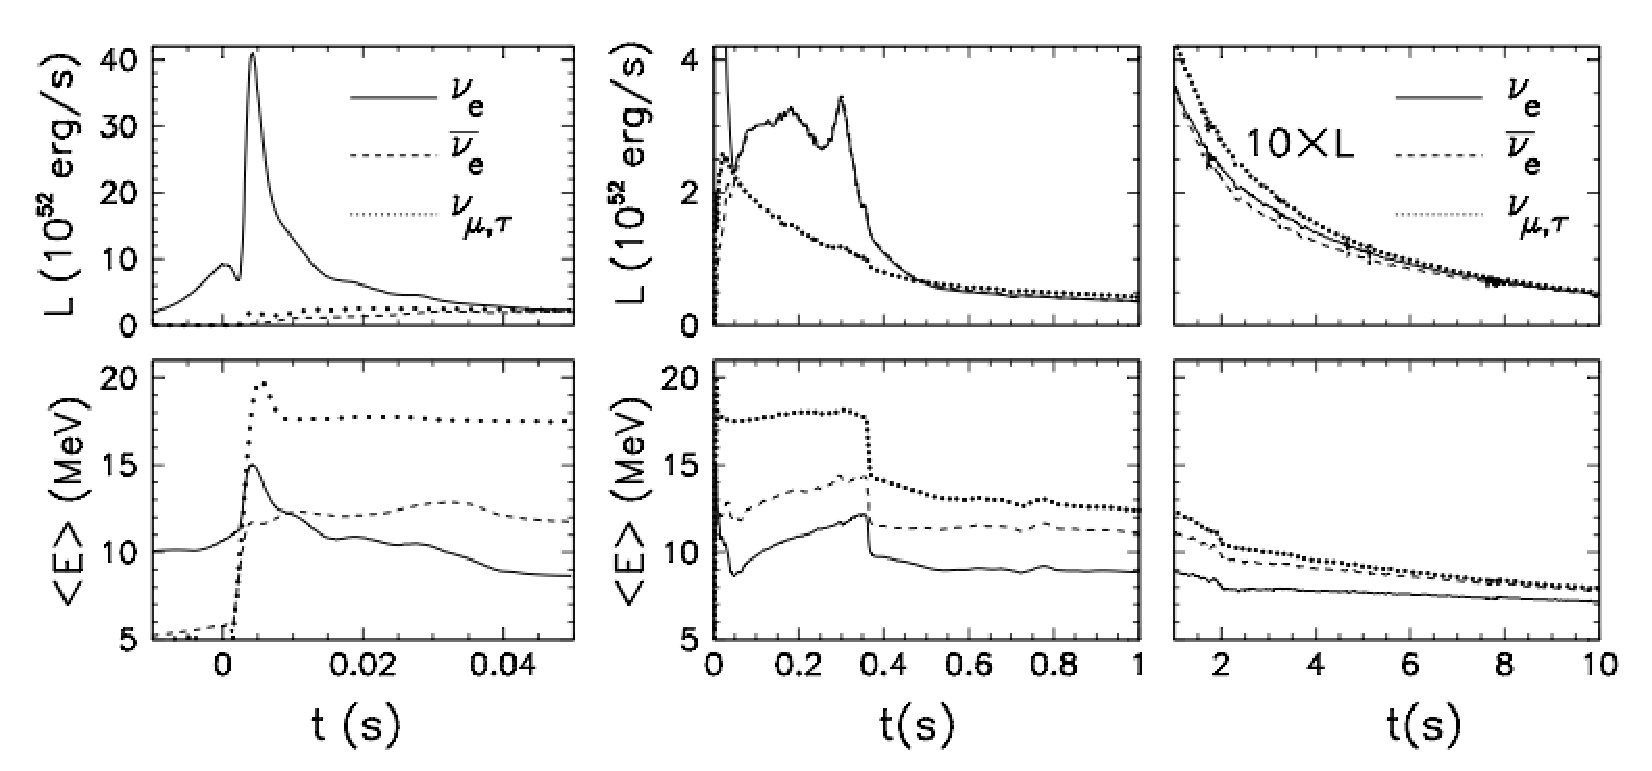
\includegraphics[width=0.9\textwidth]{basel_flux.pdf}
\caption[Expected core-collapse neutrino signal]{Expected
  core-collapse neutrino signal from the ``Basel''
  model~\cite{Fischer:2009af}, for a
  10.8 $M_{\odot}$ progenitor.  The left plots show the very early
  signal, including ``neutronization burst;'' the middle plots show
  the ``accretion phase'', and the right plots show the cooling
  phase. Across the top, luminosities as a function of time are shown. 
  Across the bottom, the plots show average energy as a function of time for the
  $\nu_e$, $\overline{\nu}_e$ and $\nu_{\mu,\tau}$ flavor components of the
  flux (fluxes for $\nu_\mu$, $\overline{\nu}_\mu$, $\nu_\tau$,
  and $\overline{\nu}_\tau$ should be identical).  Figure courtesy of~\cite{Wurm:2011zn}.}
\label{fig:spectrum}
\end{figure}

The physics of neutrino decoupling and spectra formation is far from trivial, owing to the energy dependence of the cross sections and the roles played by both charged- and neutral-current reactions. In particular, it has been argued that for $\mu$ and $\tau$ neutrinos, one should distinguish the energy sphere where these neutrinos are created and the transport sphere. Detailed transport calculations using methods such as Monte Carlo or Boltzmann solvers have been employed. It has been observed that spectra coming out of such simulations can typically be parameterized at a given moment in time by the following ansatz (e.g.,~\cite{Minakata:2008nc,Tamborra:2012ac}):
\begin{equation}
        \label{eq:pinched}
        \phi(E_{\nu}) = \mathcal{N} 
        \left(\frac{E_{\nu}}{\langle E_{\nu} \rangle}\right)^{\alpha} \exp\left[-\left(\alpha + 1\right)\frac{E_{\nu}}{\langle E_{\nu} \rangle}\right] \ ,
\end{equation}
where $E_{\nu}$ is the neutrino energy, $\langle E_\nu \rangle$ is the
mean neutrino energy, $\alpha$ is a ``pinching parameter'', and
$\mathcal{N}$ is a normalization constant.
%
Large $\alpha$ corresponds to a more ``pinched'' spectrum (suppressed
high-energy tail). This parameterization is referred to as a
``pinched-thermal'' form. The different $\nu_e$, $\overline{\nu}_e$ and
$\nu_x, \, x = \mu, \tau$ flavors are expected to have different
average energy and $\alpha$ parameters and to evolve differently in
time. 

The initial spectra get further processed (permuted) by flavor oscillations and understanding these oscillations is very important for extracting physics from the detected signal.


\subsection{Detection Channels and Interaction Rates}

Liquid argon should have a particular sensitivity to the $\nu_e$
component of a supernova neutrino burst, via charged-current
absorption of $\nu_e$ on $^{40}$Ar,
\begin{equation}
\nu_e + ^{40}{\rm Ar} \rightarrow e^- + ^{40}{\rm K^*},
\label{eq:nueabs}
\end{equation}
for which the observable is the $e^-$ as well as deexcitation products from the excited $K^*$ final state, as well as a $\bar{\nu}_e$ interaction.
  Cross sections for the most
relevant interactions are shown in Fig.~\ref{fig:xscns}.

% From Flavio
Another process of interest for supernova detection in LAr detectors, not yet fully studied,  is neutral-current  scattering on Ar nuclei by any type of neutrino: $\nu_x + Ar \rightarrow \nu_x + Ar^*$,  for which the signature is given by the cascade of de-excitation $\gamma$s from the final state Ar nucleus. A dominant 9.8-MeV Ar$^*$ decay line has been recently identified as a spin-flip M1 transition~\cite{Hayes}.   At this energy the probability of $e^+e^-$ pair production is relatively high, offering a potentially interesting neutral-current tag.
%M1 transitions are the ones that can be excited by neutrino interactions.
%  At this energy the probability of  conversion into e+,e− pair in Ar medium is nearly equivalent to Compton conversion. Identification of an e+,e− vertex from pair production of the 9.8 MeV γ looks affordable in LArTPC, providing a distinguished signature for supernova neutrino through neutral current interactions. See for example, the inset of Fig.2 where an e+,e− pair is clearly visible in an event collected with the ICARUS 3t-prototype.


\begin{figure}[!htb]
\centering
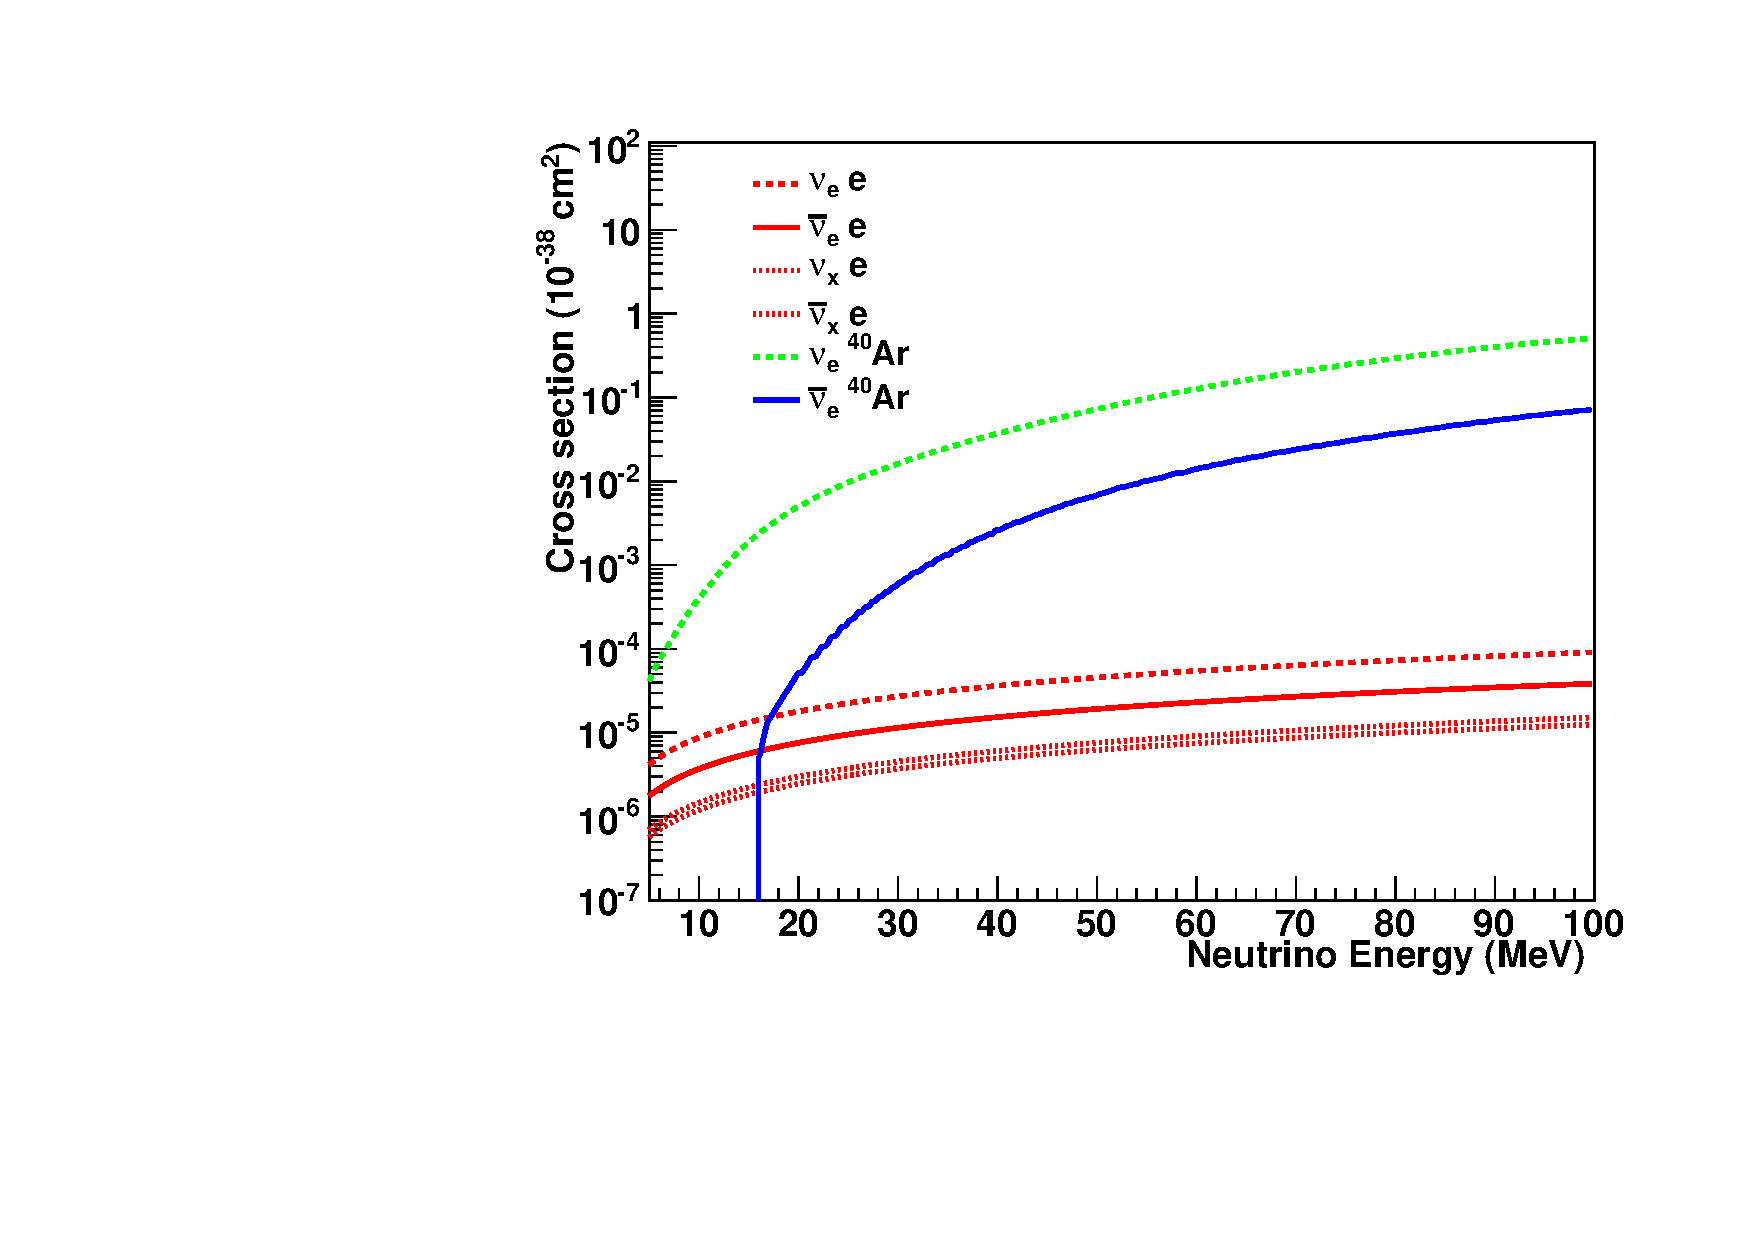
\includegraphics[width=0.6\textwidth]{argon_xscn.pdf}
\caption[]{Cross sections for supernova-relevant interactions in argon~\cite{GilBotella:2003sz,snowglobes}.}
\label{fig:xscns}
\end{figure}
%
The predicted event rate from a supernova burst may be calculated by
folding expected neutrino differential energy spectra in with cross
sections for the relevant channels, and with detector response; we do this using SNOwGLoBES~\cite{snowglobes}, which uses Icarus detector resolution~\cite{Amoruso:2003sw} and assumes a detection threshold of 5 MeV.
%


Table~\ref{tab:argon_events} shows rates calculated  for the dominant interactions in argon for
the ``Livermore'' model~\cite{Totani:1997vj} (out of date, but included for comparison with literature), and the ``GKVM''
model~\cite{Gava:2009pj}; for the former, no oscillations are assumed; the latter assumes collective effects.  In general, there is a rather wide variation--- up to an order of magnitude --- in event rate for different models, due to different numerical treatment (e.g., neutrino transport, dimensionality), physics input (nuclear equation of state, nuclear correlation and impact on neutrino opacities, neutrino-nucleus interactions), oscillation effects, in addition to intrinsic variation in the nature of the progenitor and collapse mechanism.  Neutrino emission from the supernova may furthermore be anisotropic~\cite{blah}, so that observed rates may be direction-dependent.
% Figure~\ref{fig:eventrates} shows the
%expected observed differential event spectra for these fluxes.  
%
\begin{table}[!htb]
  \caption[Event rates for different models in \SI{34}{\kt} of LAr for
    a core-collapse at 10~kpc]{Event rates for different
    supernova models in \SI{34}{\kt} of liquid argon for a core collapse at 10~kpc, for $\nu_e$ and $\bar{\nu}_e$ charged-current channels and elastic scattering (ES) on electrons.
    Event rates will simply scale by active detector mass and inverse square of supernova distance.   No oscillations are assumed; we note that oscillations (both standard and ``collective'') will potentially have a large, model-dependent effect. \fixme{Update to 40 kt}}
\label{tab:argon_events}\centering
\begin{tabular}{$L^c^c}%$
\toprule
\rowtitlestyle
Channel & Events & Events \\
\rowtitlestyle
& ``Livermore'' model & ``GKVM'' model  \\ 
\toprowrule

$\nu_e + ^{40}{\rm Ar} \rightarrow e^- + ^{40}{\rm K^*}$ & 2308  & 2848 \\ \colhline

$\overline{\nu}_e + ^{40}{\rm Ar} \rightarrow e^+ + ^{40}{\rm Cl^*}$ & 194 & 134\\ \colhline

$\nu_x + e^- \rightarrow \nu_x + e^-$                           & 296 &  178\\

%$\nu_x + ^{40}{\rm Ar} \rightarrow \nu_x+ ^{40}{\rm Ar}^*$ & & \\ \hline
\toprule
\rowtitlestyle
Total &  2794& 3160 \\ 
\bottomrule
\end{tabular}
\end{table}

%
% \begin{figure}[!htb]
% \centering
% 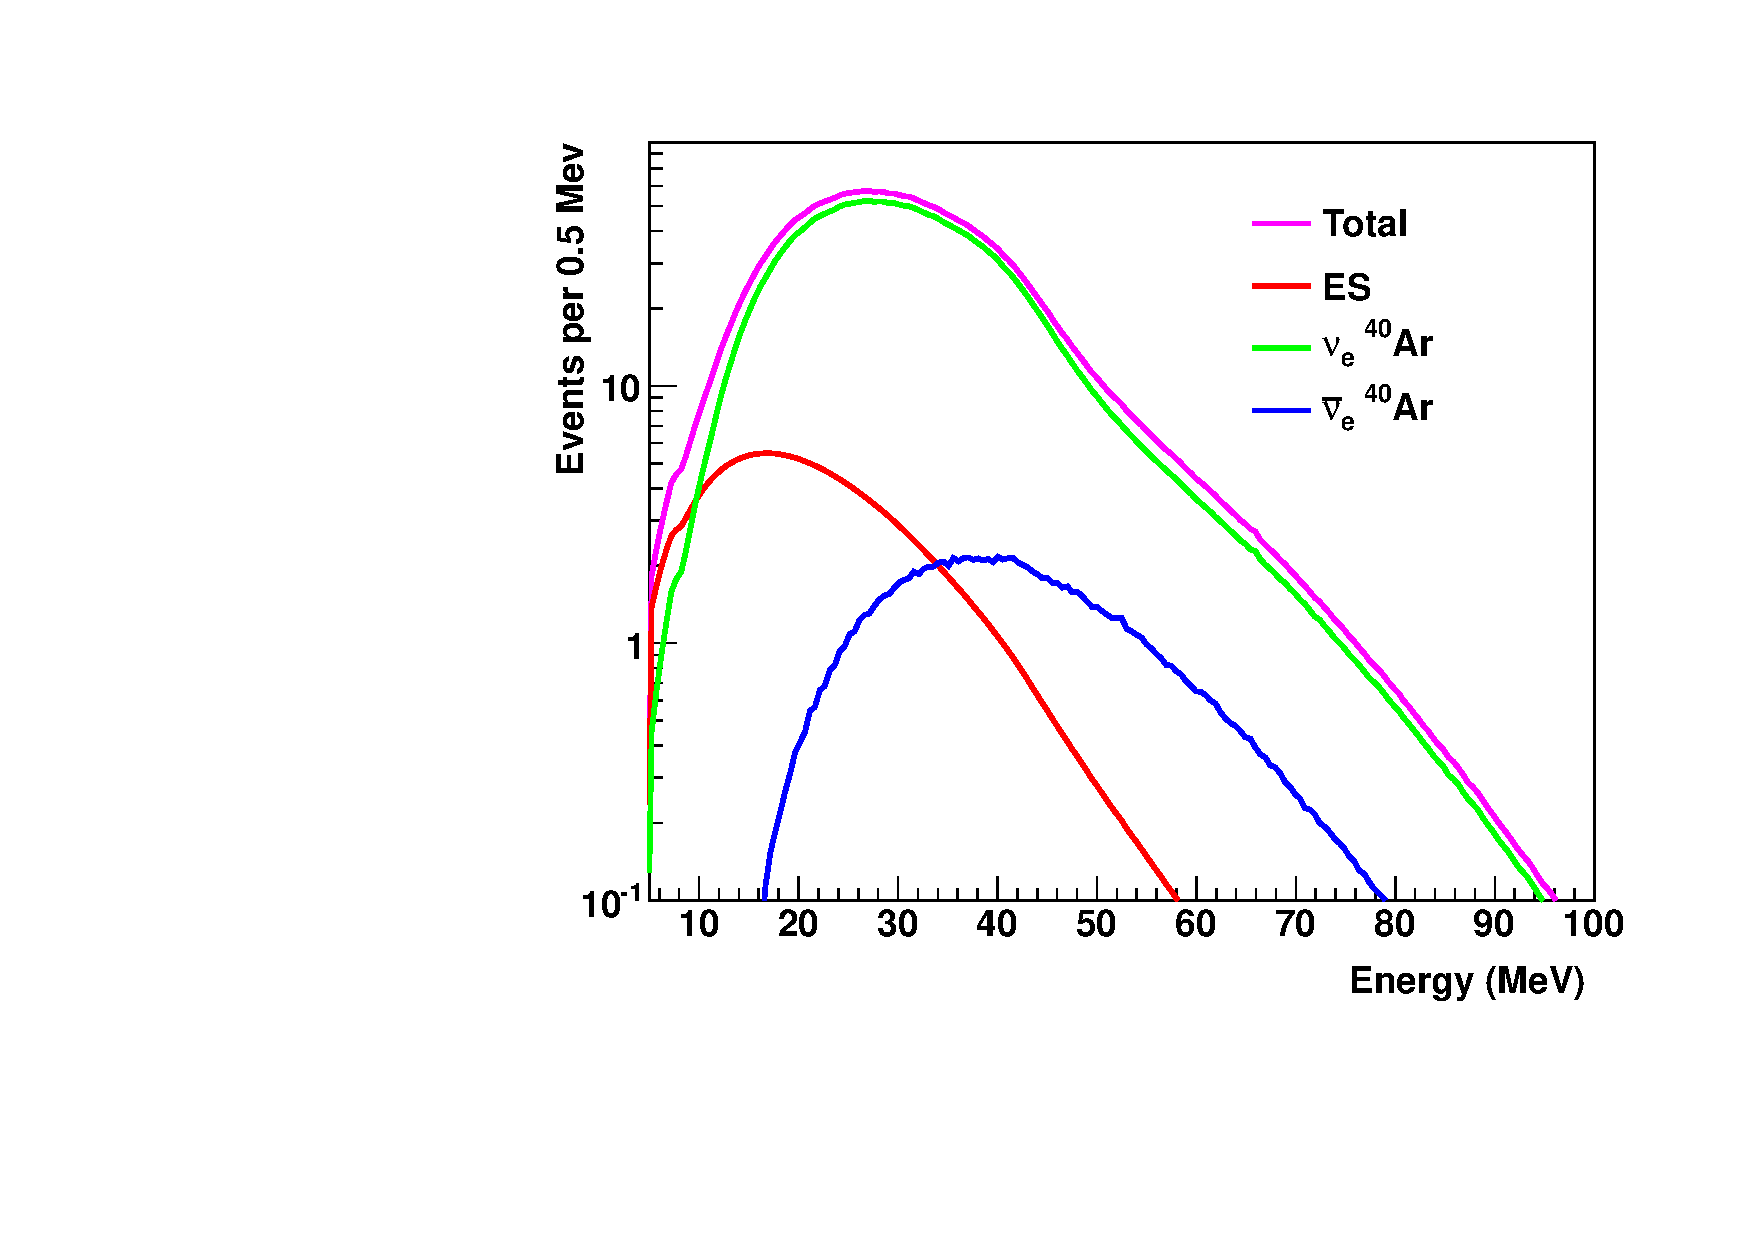
\includegraphics[width=2.0in]{interaction_rates_gvkm_ar34kt.pdf}
% 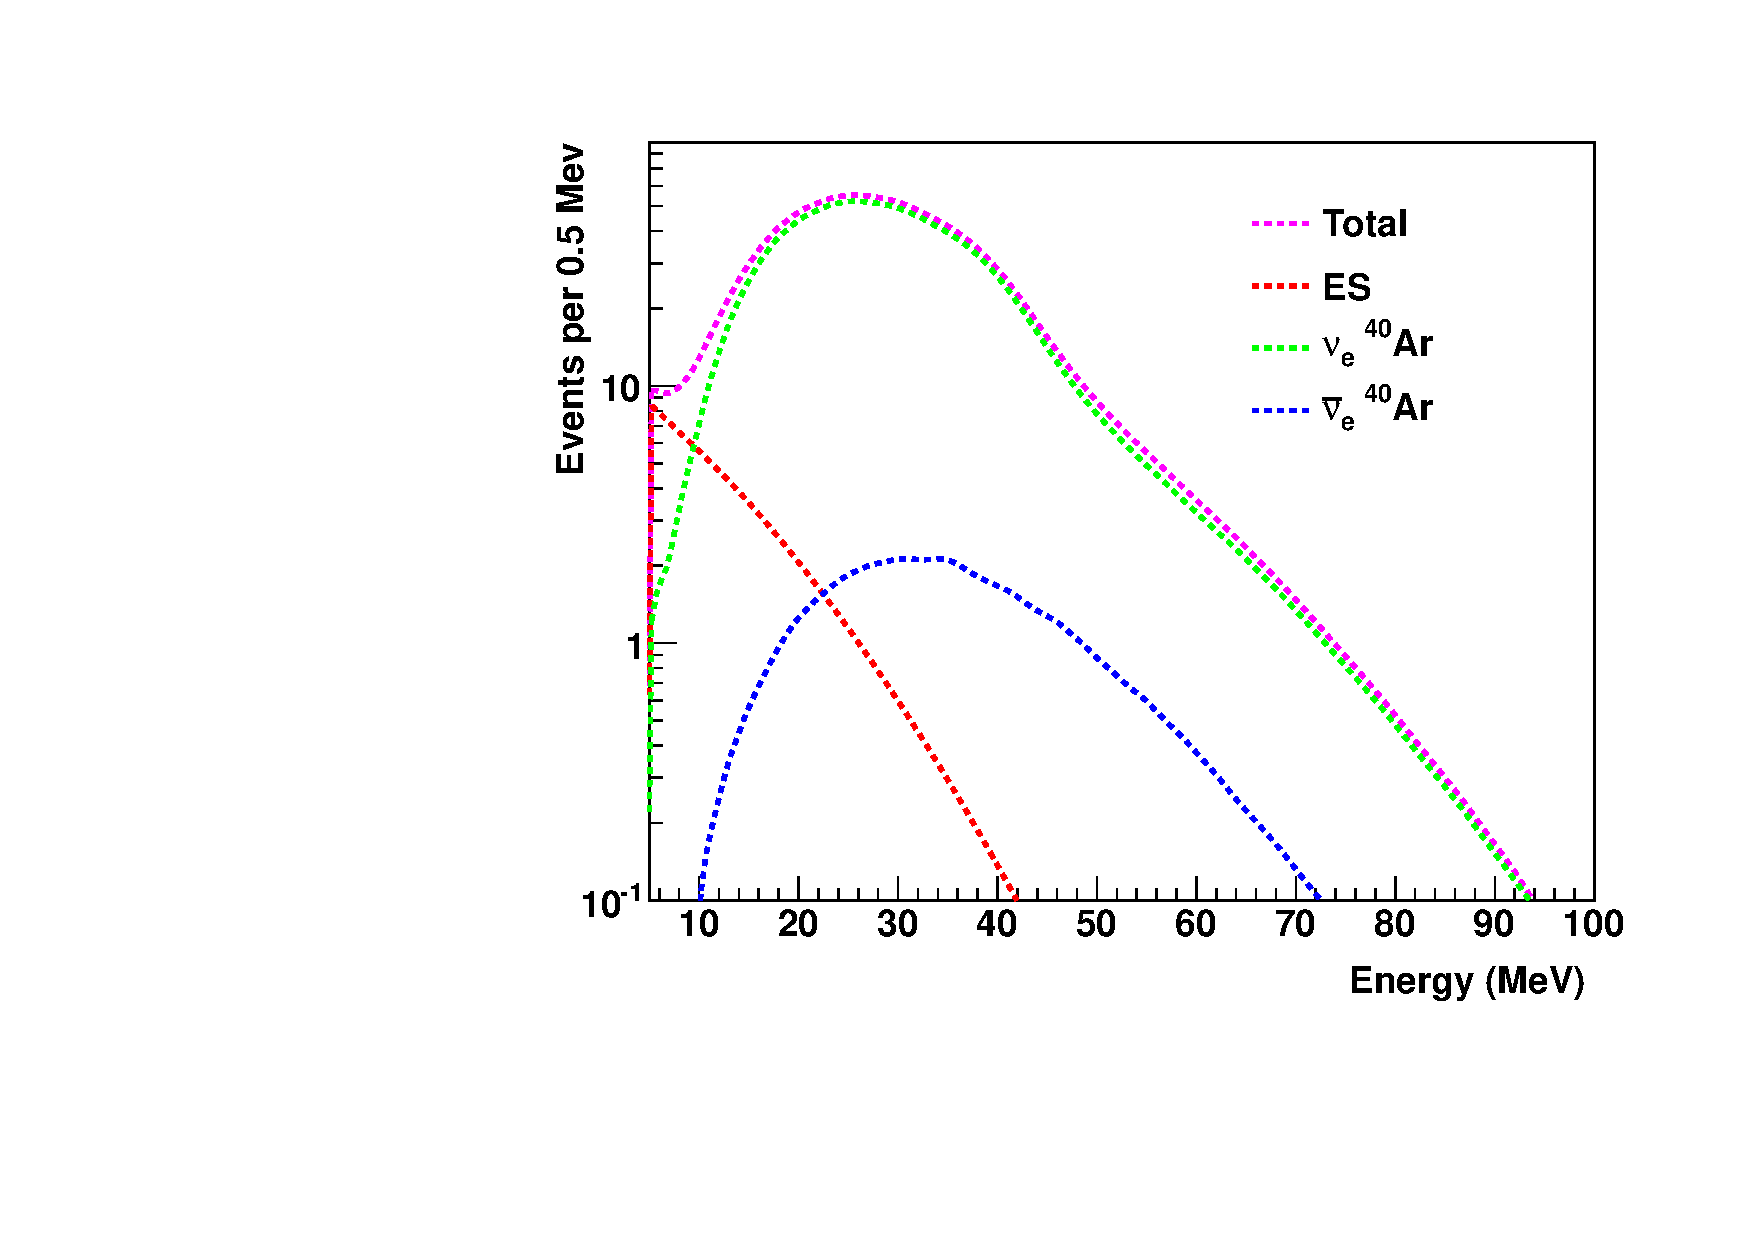
\includegraphics[width=2.0in]{smeared_rates_gvkm_ar34kt.pdf}
% \vspace{-5pt}
% \caption[SN $\nu$ event rates in \SI{34}{kt} of LAr for a core
%   collapse at 10~kpc, GKVM]{Supernova neutrino event rates in 34~kt of argon for a core
%   collapse at 10~kpc, for the GKVM model~\cite{Gava:2009pj} (events
%   per 0.5~MeV), showing three relevant interaction channels. Left:
%   interaction rates as function of true neutrino energy.  Right:
%   ``smeared'' rates as a function of detected energy, assuming
%   resolution from~\cite{Amoruso:2003sw}.}
%   \label{fig:eventrates}
% \end{figure}


Figure~\ref{fig:garching} gives another example of an expected burst
signal, for which a calculation with detailed time dependence of the
spectra is available~\cite{Huedepohl:2009wh} out to 9~seconds
post-bounce.  This model has relatively low luminosity but the standard robust
neutronization burst.  Note that the relative fraction of
neutronization-burst events is quite high.
Figure~\ref{fig:eventrates} shows the event channel breakdown for the same model.  Clearly, the $\nu_e$
flavor dominates.

%
\begin{figure}[!htb]
\centering
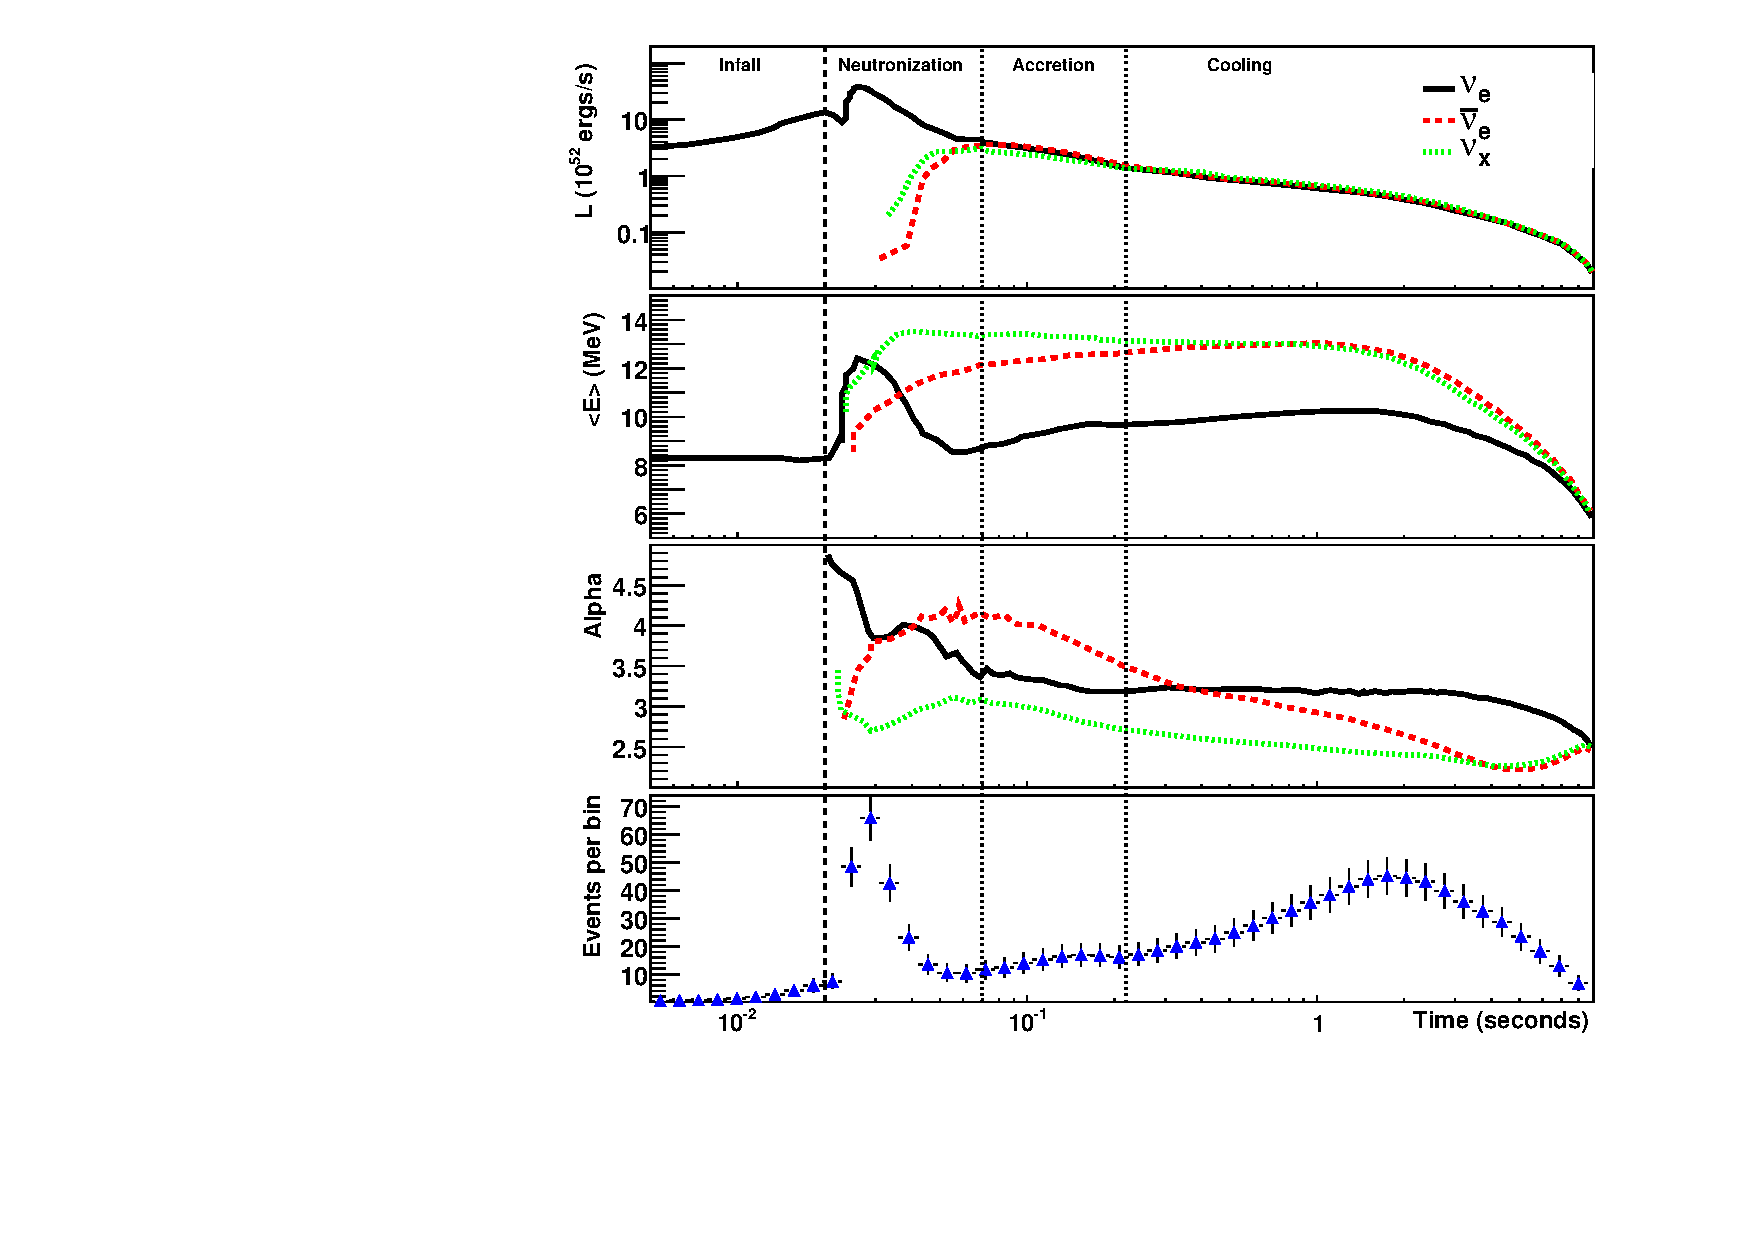
\includegraphics[width=0.9\textwidth]{garching.pdf}
\caption[Garching flux signal with neutronization burst]{ Expected
  time-dependent signal for a specific flux model for an
  electron-capture supernova~\cite{Huedepohl:2009wh} at 10~kpc.  No oscillations are assumed. The
  top plot shows the luminosity as a function of time, the second plot
  shows average neutrino energy, and the third plot shows the $\alpha$
  (pinching) parameter.  The fourth (bottom) plot shows the total number of
  events (mostly $\nu_e$) expected in 34 kt of liquid argon, calculated using
  SNOwGLoBES.  Note the logarithmic binning in time; the plot shows
  the number of events expected in the given bin and the error bars
  are statistical. The vertical dashed line at 0.02 seconds indicates
  the time of core bounce, and the vertical lines indicate different
  eras in the supernova evolution.  The leftmost time interval
  indicates the infall period.  The next interval, from core bounce to
  50~ms, is the neutronization burst era, in which the flux is
  composed primarily of $\nu_e$.  The next period, from 50 to 200~ms,
  is the accretion period. The final era, from 0.2 to 9~seconds, is
  the proto-neutron-star cooling period.  \fixme{Update to 40 kt}}
\label{fig:garching}
\end{figure}


\begin{figure}[!htb]
\centering
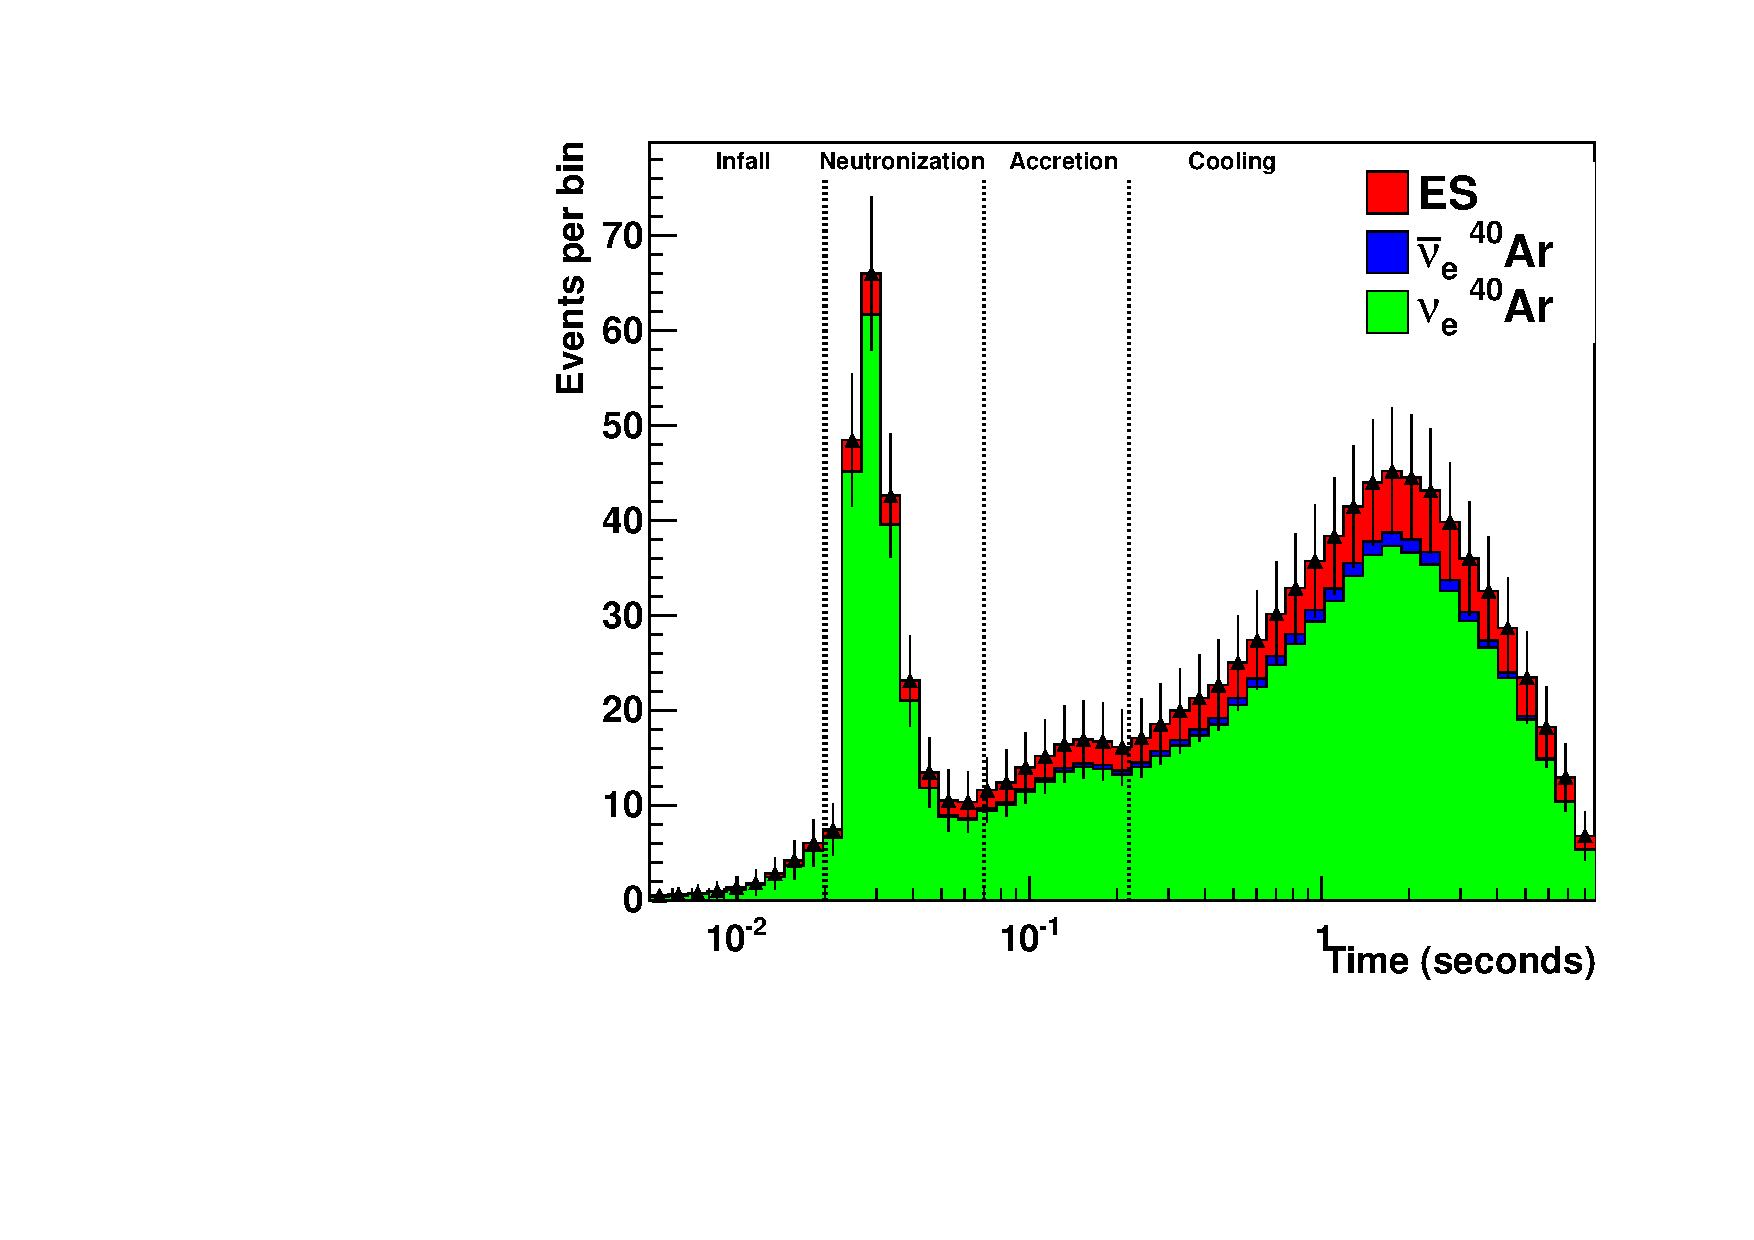
\includegraphics[width=2.5in]{garching_time_plot.pdf}
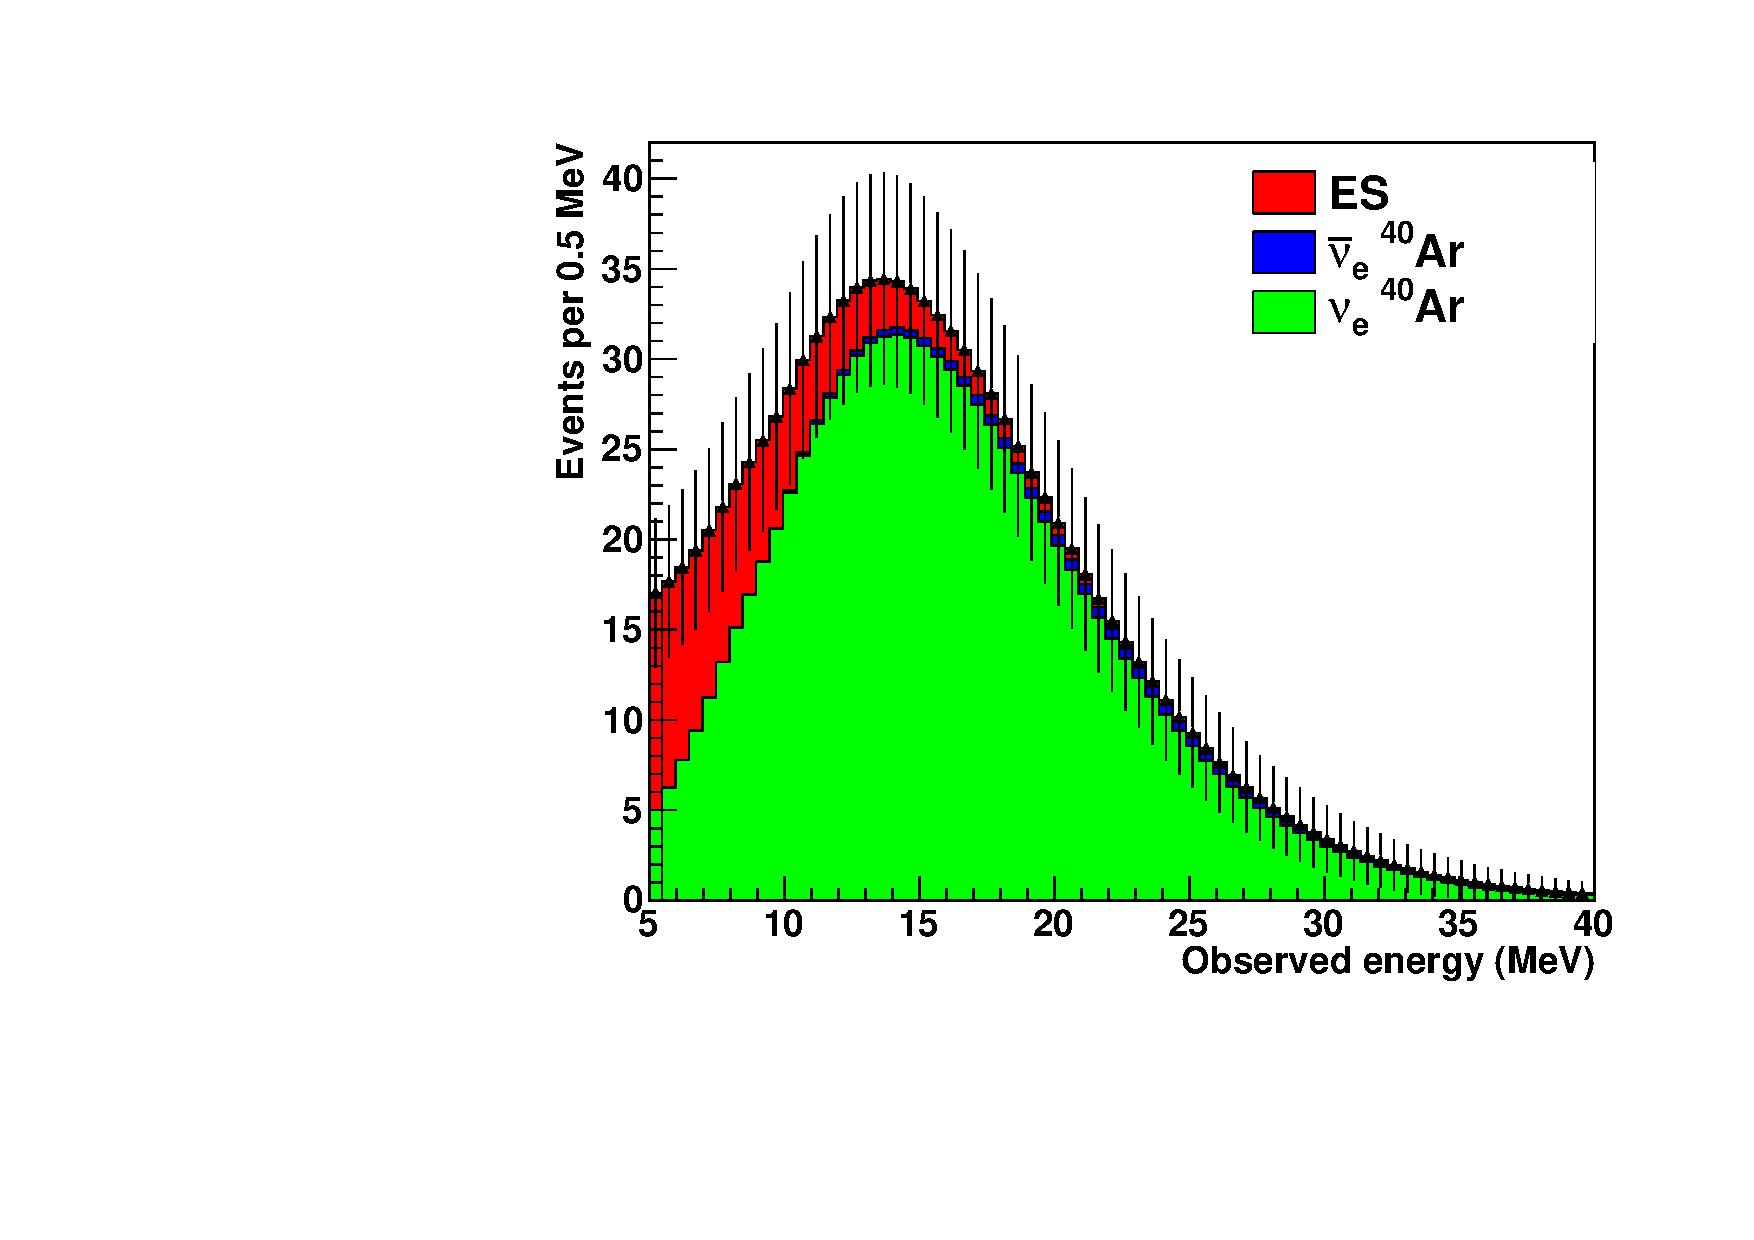
\includegraphics[width=2.5in]{garching_energy_plot.pdf}
\vspace{-5pt}
\caption[Supernova $\nu$ event rates in \SI{40}{kt} of LAr for Garching flux]{Left: Expected
  time-dependent signal in 40 kt of liquid argon for the electron-capture supernova~\cite{Huedepohl:2009wh} at 10~kpc, calculated using SNoWGLoBES~\cite{snowglobes}, showing breakdown of event channels.  Right: expected measured event spectrum for the same model, integrated over time.}

  \label{fig:eventrates}
\end{figure}

The number of signal events scales with mass and inverse square of distance as shown in Fig.~\ref{fig:ratesvsdist}.  For a collapse in the Andromeda galaxy, a 40-kton detector would observe a few events.

\begin{figure}[!htb]
\centering
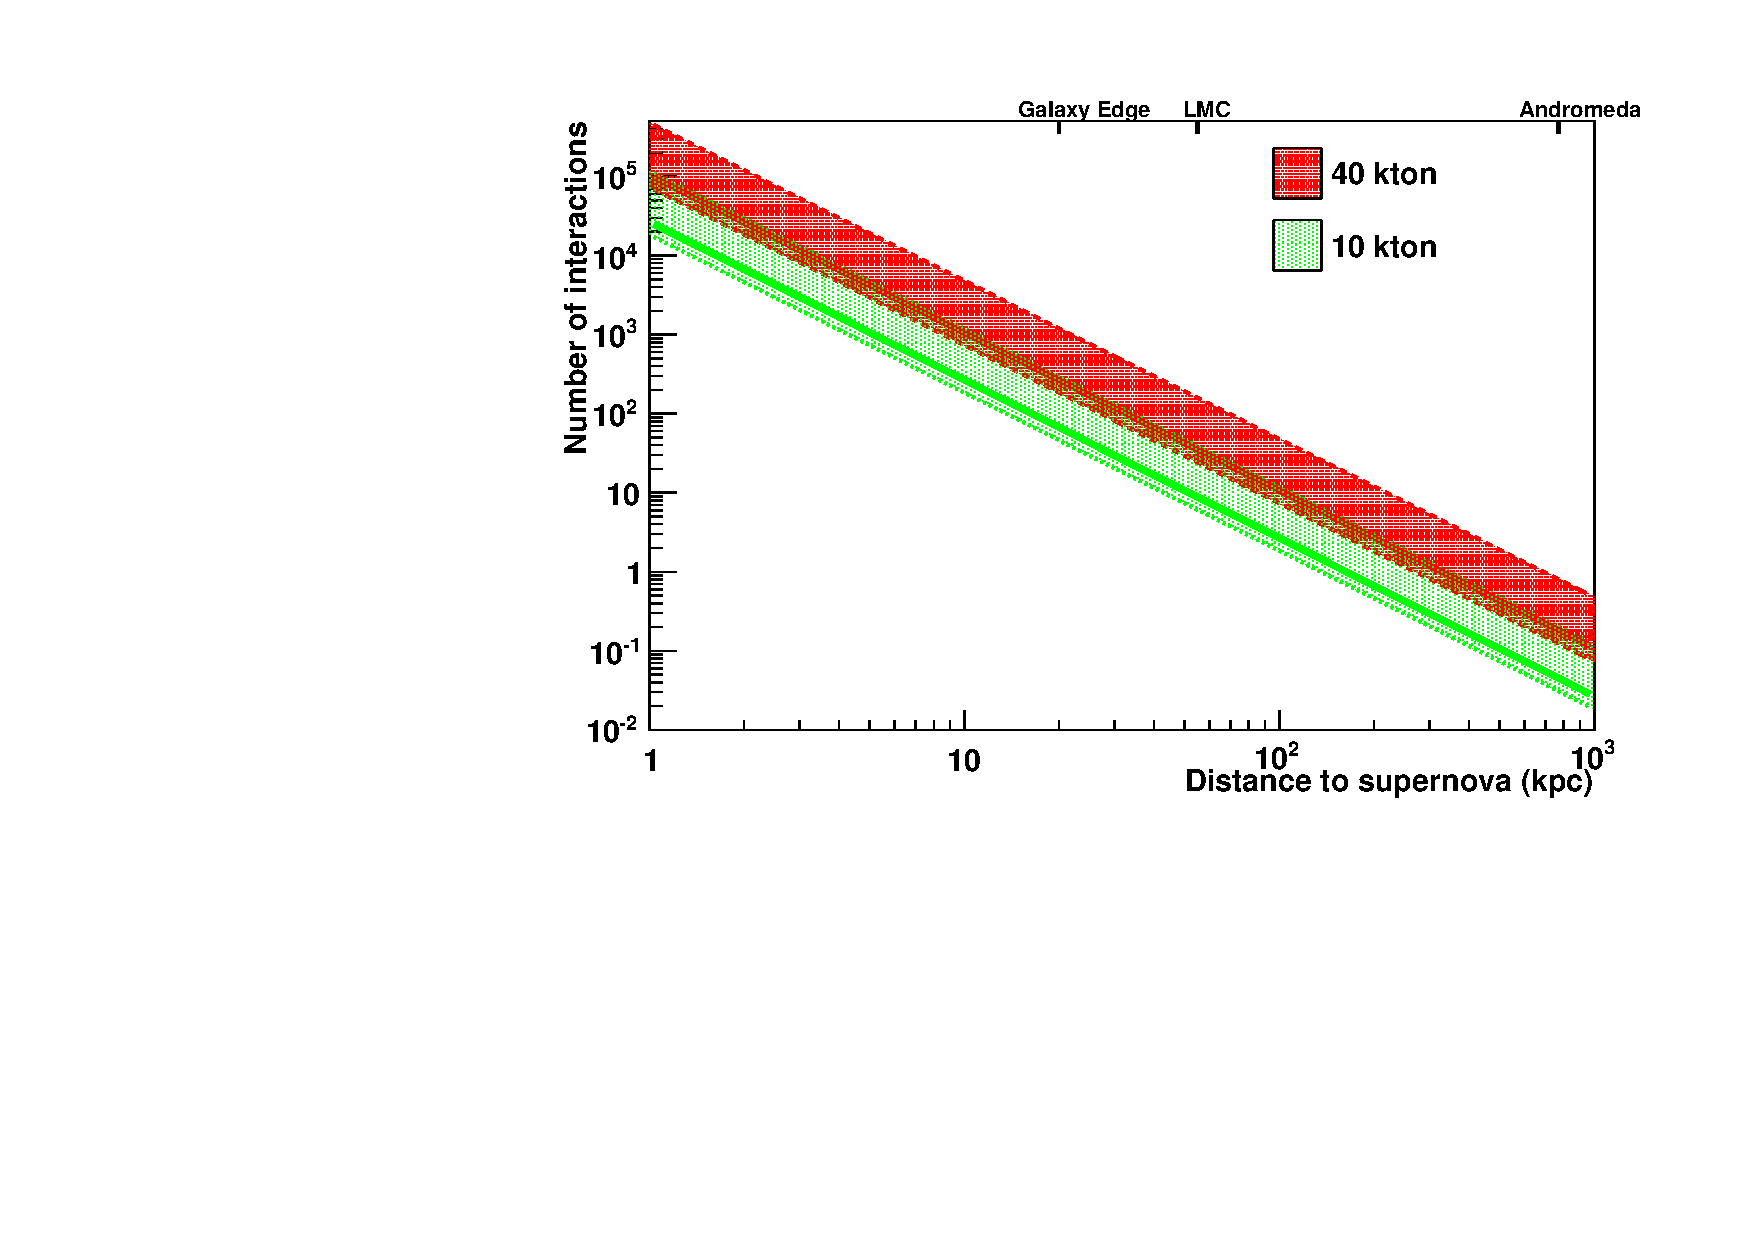
\includegraphics[width=5in]{argon_sn.pdf}
\caption[Rates vs distance]{Estimated numbers of supernova neutrino interactions in DUNE as a function of distance to the supernova, for different detector masses ($\nu_e$ events dominate). The red dashed lines represent expected events for a 40-kton detector and the green dotted lines represent expected events for a 10-kton detector. The lines limit a fairly wide range of possibilities for ``Garching-parameterized'' supernova flux spectra with luminosity $0.5\times 10^{52}$ ergs over ten seconds. The optimistic upper line of a pair gives the number of events for average $\nu_e$ energy of $\langle E_{\nu_e}\rangle =12$~MeV, and ``pinching'' parameter $\alpha=2$; the pessimistic lower line of a pair gives the number of events for $\langle E_{\nu_e}\rangle=8$~MeV and $\alpha=6$. (Note that the luminosity, average energy and pinching parameters will vary over the time frame of the burst, and these estimates assume a constant spectrum in time. Oscillations will also affect the spectrum and event rates.) The solid lines represent the integrated number of events for the specific time-dependent neutrino flux model in~\cite{Huedepohl:2009wh} (see Figs.~\ref{fig:garching} and \ref{fig:eventrates}; this model has relatively cool spectra and low event rates). Core collapses are expected to occur a few times per century, at a most-likely distance of around 10 to 15 kpc.}

  \label{fig:ratesvsdist}
\end{figure}



\section{Neutrino Physics and Other Particle Physics}
\label{sec:physics-snblowe-neutrino-physics}

As already mentioned, a core-collapse supernova is essentially a gravity-powered neutrino bomb: the energy of the collapse is initially stored in the Fermi seas of electrons and neutrinos and then gradually leaked out by neutrino diffusion. The key property of neutrinos that makes them play such a dominant role in the supernova dynamics is the feebleness of their interactions. It then follows that should there be new light ($< 100$ MeV) particles with even weaker interactions, they could alter the energy transport process and the resulting evolution of the nascent proto-neutron star. Moreover, additional interactions or properties of neutrinos could also be manifested in this way. 

Thus, a core-collapse supernova can therefore be thought of as an extremely hermetic system, which can be used to search for numerous types of new physics (e.g., ~\cite{Raffelt:1999tx}). The list includes various Goldstone bosons (e.g., Majorons), neutrino magnetic moments, new gauge bosons (``dark photons''), ``unparticles'', and extra-dimensional gauge bosons. The existing data from SN1987A already provides significant constraints on these scenarios, by confirming the basic energy balance of the explosion. At the same time, more precision is highly desirable and should be provided with the next galactic supernova. 

\begin{figure}[!htb]
\centering
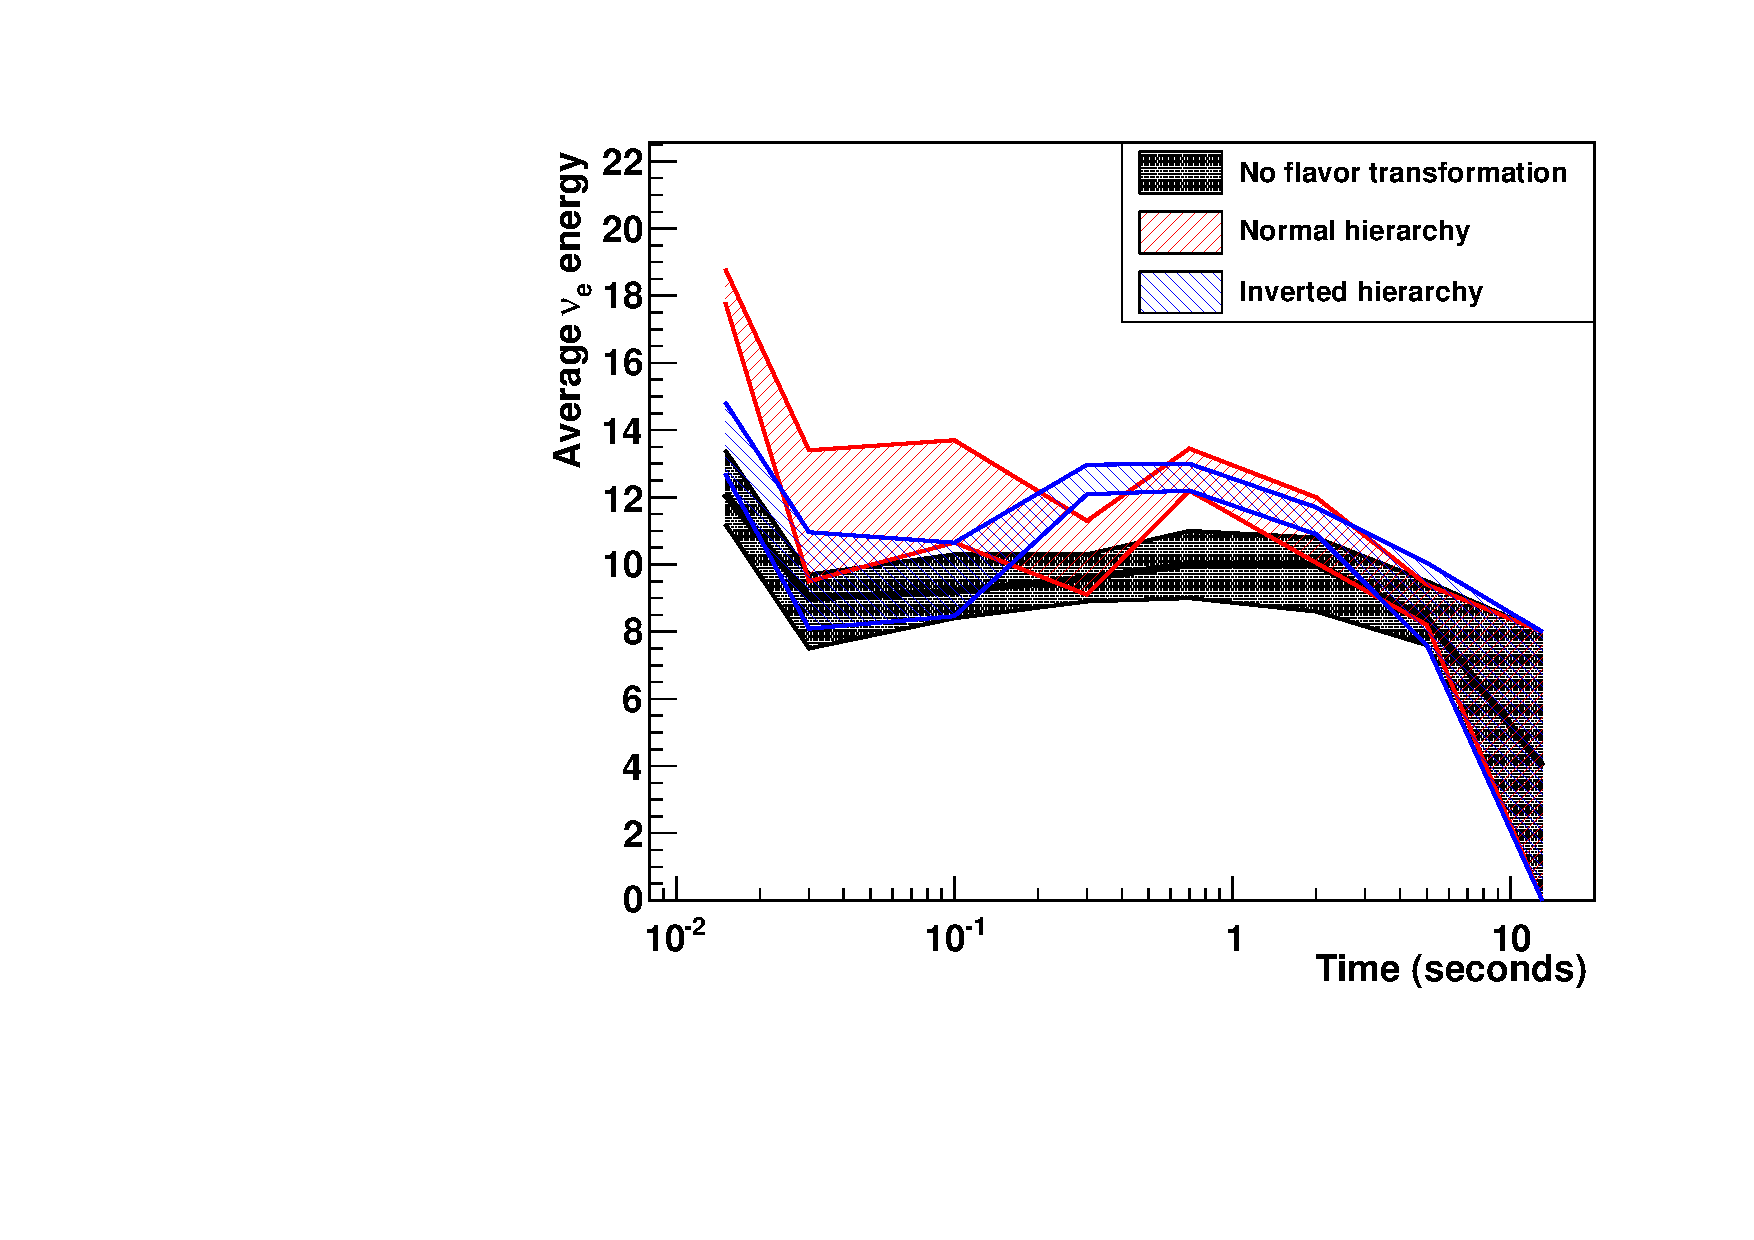
\includegraphics[width=0.9\textwidth]{timedep.pdf}
\caption[Simulated cooling curves from the Garching light progenitor model]{ Average $\nu_{e}$ energy from a simulated fit to the oscillated fluxes predicted by the Garching 1D model with a light (10.8 $M_{\odot}$) progenitor. Our oscillation calculations included full multi-angle treatment of collective evolution, for two
different mass hierarchy assumptions. The predicted events were then smeared with SNOwGLoBES and fit with pinched-thermal spectrum as a function of time (assuming a supernova at 10 kpc and a 34 kt LAr detector). The bands represent $1\sigma$ error bars from the fit (assuming only statistical uncertainties). The solid black line is the true
$\langle E_{\nu} \rangle$ for the unoscillated spectrum. Clearly, the rate of energy escape from the proto-neutron star can be gleaned by tracking $\nu_{e}$ spectra as a function of time.}
\label{fig:coolingcurves}
\end{figure}


The analysis will make use of two types of information. First, the total energy of the emitted neutrinos should be compared with the expected release in the gravitational collapse. Examples of the integrated neutrino event rates are shown in Fig.~\ref{fig:eventrates}. Second, the rate of cooling of the protoneutron state should be measured and compared with what is expected from diffusion of the standard neutrinos. This requires comparing one-second-interval time-integrated spectra at successive times as illustrated in Fig.~\ref{fig:coolingcurves}. 

Each of these methods on its own is subject to certain subtleties and limitations. For example, the total energy release occurs in all flavors, while the DUNE detector will be mostly sensitive to electron neutrinos, as seen in Fig.~\ref{fig:eventrates}. Additional data and theoretical analysis will be necessary; for example, the complementary data from the water Cherenkov detector for the measurement of $\bar\nu_{e}$ and a careful analysis of the oscillation pattern (see below) to infer the fluxes of $\mu$ and $\tau$ flavors. As for measuring the energy loss rate, it will require sufficient statistics at late times and, once again, understanding the oscillation dynamics, as is clear in Fig.~\ref{fig:coolingcurves} where oscillated and unoscillated cases are shown.

This brings us to the second major part of the science program, namely, the flavor oscillation physics and its signatures. Compared to the well-understood case of solar neutrinos, in a supernova neutrino flavor transformations are much more involved. Not only neutrinos and antineutrinos of all flavors are emitted, not only are there two mass splittings -- ``solar'' and ``atmospheric'' -- to worry about, but the physics of the transformations is significantly richer. For example, several seconds after the onset of the explosion, the flavor conversion probability is affected by the expanding shock front and the turbulent region behind it. The conversion process in such a stochastic profile is qualitatively different from the adiabatic MSW effect in the smooth, fixed density profile of the Sun. 

Even more complexity is brought about by the coherent scattering of neutrinos off each other. This neutrino ``self-refraction'' 
 results in highly nontrivial flavor transformations close to the neutrinosphere, typically within a few hundred kilometers from the center, where the density of streaming neutrinos is very high. Since the evolving flavor composition of the neutrino flux feeds back into the oscillation Hamiltonian, the problem is \emph{nonlinear}. Furthermore, as the interactions couple neutrinos and antineutrinos of different flavors and energies, the oscillations are characterized by \emph{collective} modes. This leads to very rich physics that has been the subject of intense interest over the last decade and a voluminous literature exists exploring these collective phenomena,
e.g.,~\cite{Duan:2005cp,Fogli:2007bk,Raffelt:2007cb,Raffelt:2007xt,EstebanPretel:2008ni,Duan:2009cd,Dasgupta:2009mg,Duan:2010bg,Duan:2010bf,Wu:2014kaa}.  This is an active theoretical field and the effects are not yet fully understood.
Matter effects in the Earth can also have an effect on the signal~\cite{Choubey:2010up}.
\fixme{More references here, update}

\begin{figure}[!htb]
\centering
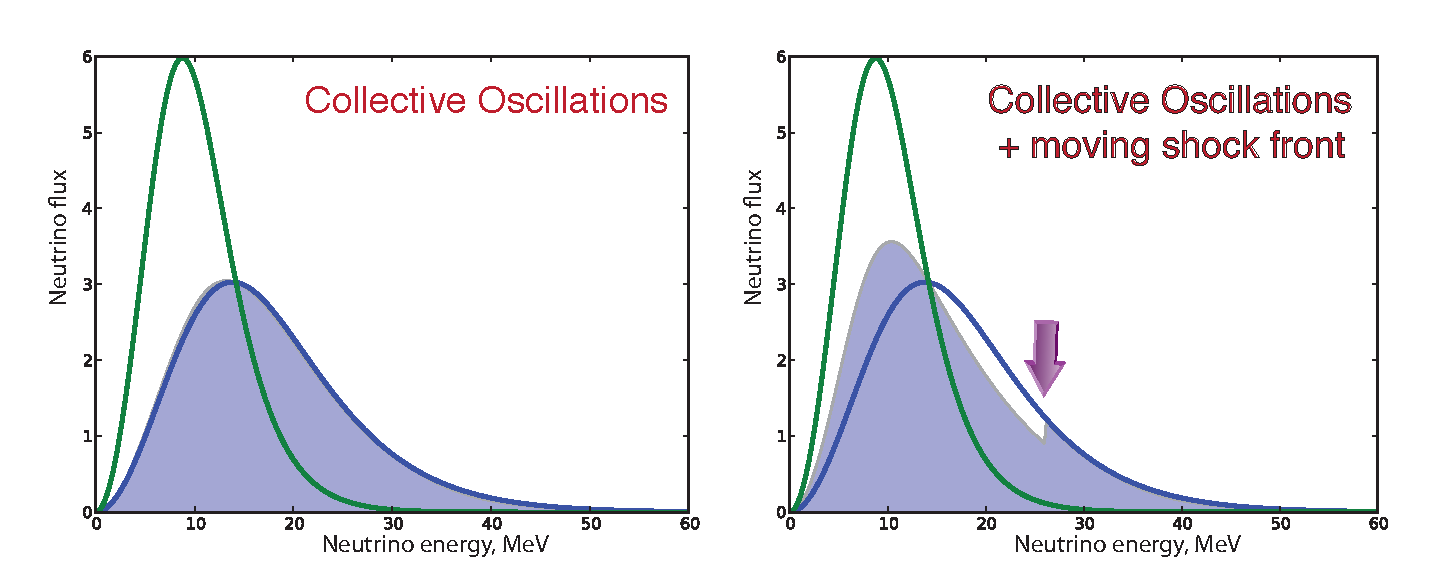
\includegraphics[width=0.9\textwidth]{shockandcollective.pdf}
\caption[Simulated cooling curves from the Garching light progenitor model]{ A simulation of the effects of collective oscillations alone (left panel) and of collective oscillations plus the shock front (right panel).}
\label{fig:shockandcollective}
\end{figure}

One may wonder whether all this complexity will impede the extraction of useful information from the future signal. In fact, the opposite is true: the new effects can \emph{imprint} information about the inner workings of the explosion on the signal. The oscillations can modulate the characteristics of the signal (both event rates and spectra as a function of time), as seen in Fig.~\ref{fig:coolingcurves}. Moreover, the oscillations can imprint \emph{non-thermal} features on the energy spectra, potentially making it possible to disentangle the effects of flavor transformations and the physics of neutrino spectra formation. This in turn should help us learn about the development of the explosion during the crucial first 10 seconds.   It is important to note that the features depend on the unknown mass hierarchy, and so can potentially tell us what the hierarchy is.

An illustration is provided in Fig.~\ref{fig:shockandcollective}. The role of the collective oscillations in this case is to almost completely permute the original $\nu_{e}$ and $\nu_{\mu,\tau}$ spectra, so that the flux of observed electron neutrinos is noticeably hotter than the original one. Moreover, the shock front modulated the MSW conversion probability and imprints a nonthermal ``step'' in the spectrum. Below this step, the swap between the original $\nu_{e}$ and $\nu_{\mu,\tau}$ spectra is only partial. As the shock expands, the feature moves to higher energies, creating a ``smoking-gun'' signature that exists only in the neutrino channel. 



% Neutrino oscillations modulate the flavor-energy-time evolution of the spectrum, including 
% ``collective'' effects due to neutrino-neutrino interactions.  A
% voluminous literature exists exploring these collective phenomena,
% e.g.,~\cite{Duan:2005cp,Fogli:2007bk,Raffelt:2007cb,Raffelt:2007xt,EstebanPretel:2008ni,Duan:2009cd,Dasgupta:2009mg,Duan:2010bg,Duan:2010bf}.



% Certain phenomena are even postulated to indicate
% beyond-the-standard-model physics~\cite{Raffelt:1999tx} such as
% axions, extra dimensions and an anomalous neutrino magnetic moment;
% non-observation of these effects, conversely, would enable constraints
% on these phenomena.


%\textit{Add: absolute mass?}


% From Alan Kostelecky
As another example of a probe of new physics with supernova neutrinos or antineutrinos,
% neutrino oscillations offer observable signals for Lorentz and CPT violation because they compare the propagation of two flavors. 
a class of tests of Lorentz and CPT violation involves comparing the propagation of neutrinos with other species or of neutrinos of the same flavor but different energies~\cite{Kostelecky:2003cr,Kostelecky:2003xn,Kostelecky:2011gq,Diaz:2009qk}. These amount to time-of-flight or dispersion studies.
Time-of-flight and dispersion effects lack the interferometric resolving power available to neutrino oscillations, but they provide instead sensitivity to Lorentz- and CPT-violating effects that cannot be detected via oscillations. The corresponding SME coefficients controlling these effects are called oscillation-free coefficients~\cite{Kostelecky:2011gq}.
Supernova neutrinos are of particular interest in this context because of the long baseline, which implies sensitivities many orders of magnitude better than available from time-of-flight measurements in beams. Observations of the supernova SN1987A yield constraints on the difference between the speed of light and the speed of antineutrinos, which translates into constraints on isotropic and anisotropic coefficients in both the minimal and nonminimal sectors of the SME. Knowledge of the spread of arrival times constrains the maximum speed difference between SN1987A antineutrinos of different energies in the approximate range 10-40 MeV, which restricts the possible antineutrino dispersion and yields further constraints on SME coefficients~\cite{Kostelecky:2011gq}.
Analyses of this type would be possible with DUNE if supernova neutrinos are observed. Key features to maximize sensitivity would include absolute timing information to compare with photon spectral observations and relative timing information for different components of the antineutrino energy spectrum. Significant improvements over existing limits are possible.
Figure 4 displays DUNE supernova sensitivities to coefficients for Lorentz and CPT violation that leave unaffected neutrino oscillations and so cannot be measured using atmospheric or long-baseline neutrinos. The figure assumes a supernova comparable to SN1987A (optimistically at a distance of 50 kpc). Studies of supernova neutrinos using DUNE can measure many coefficients (green) at levels improving over existing limits (grey).

\begin{figure}[!htb]
\centering
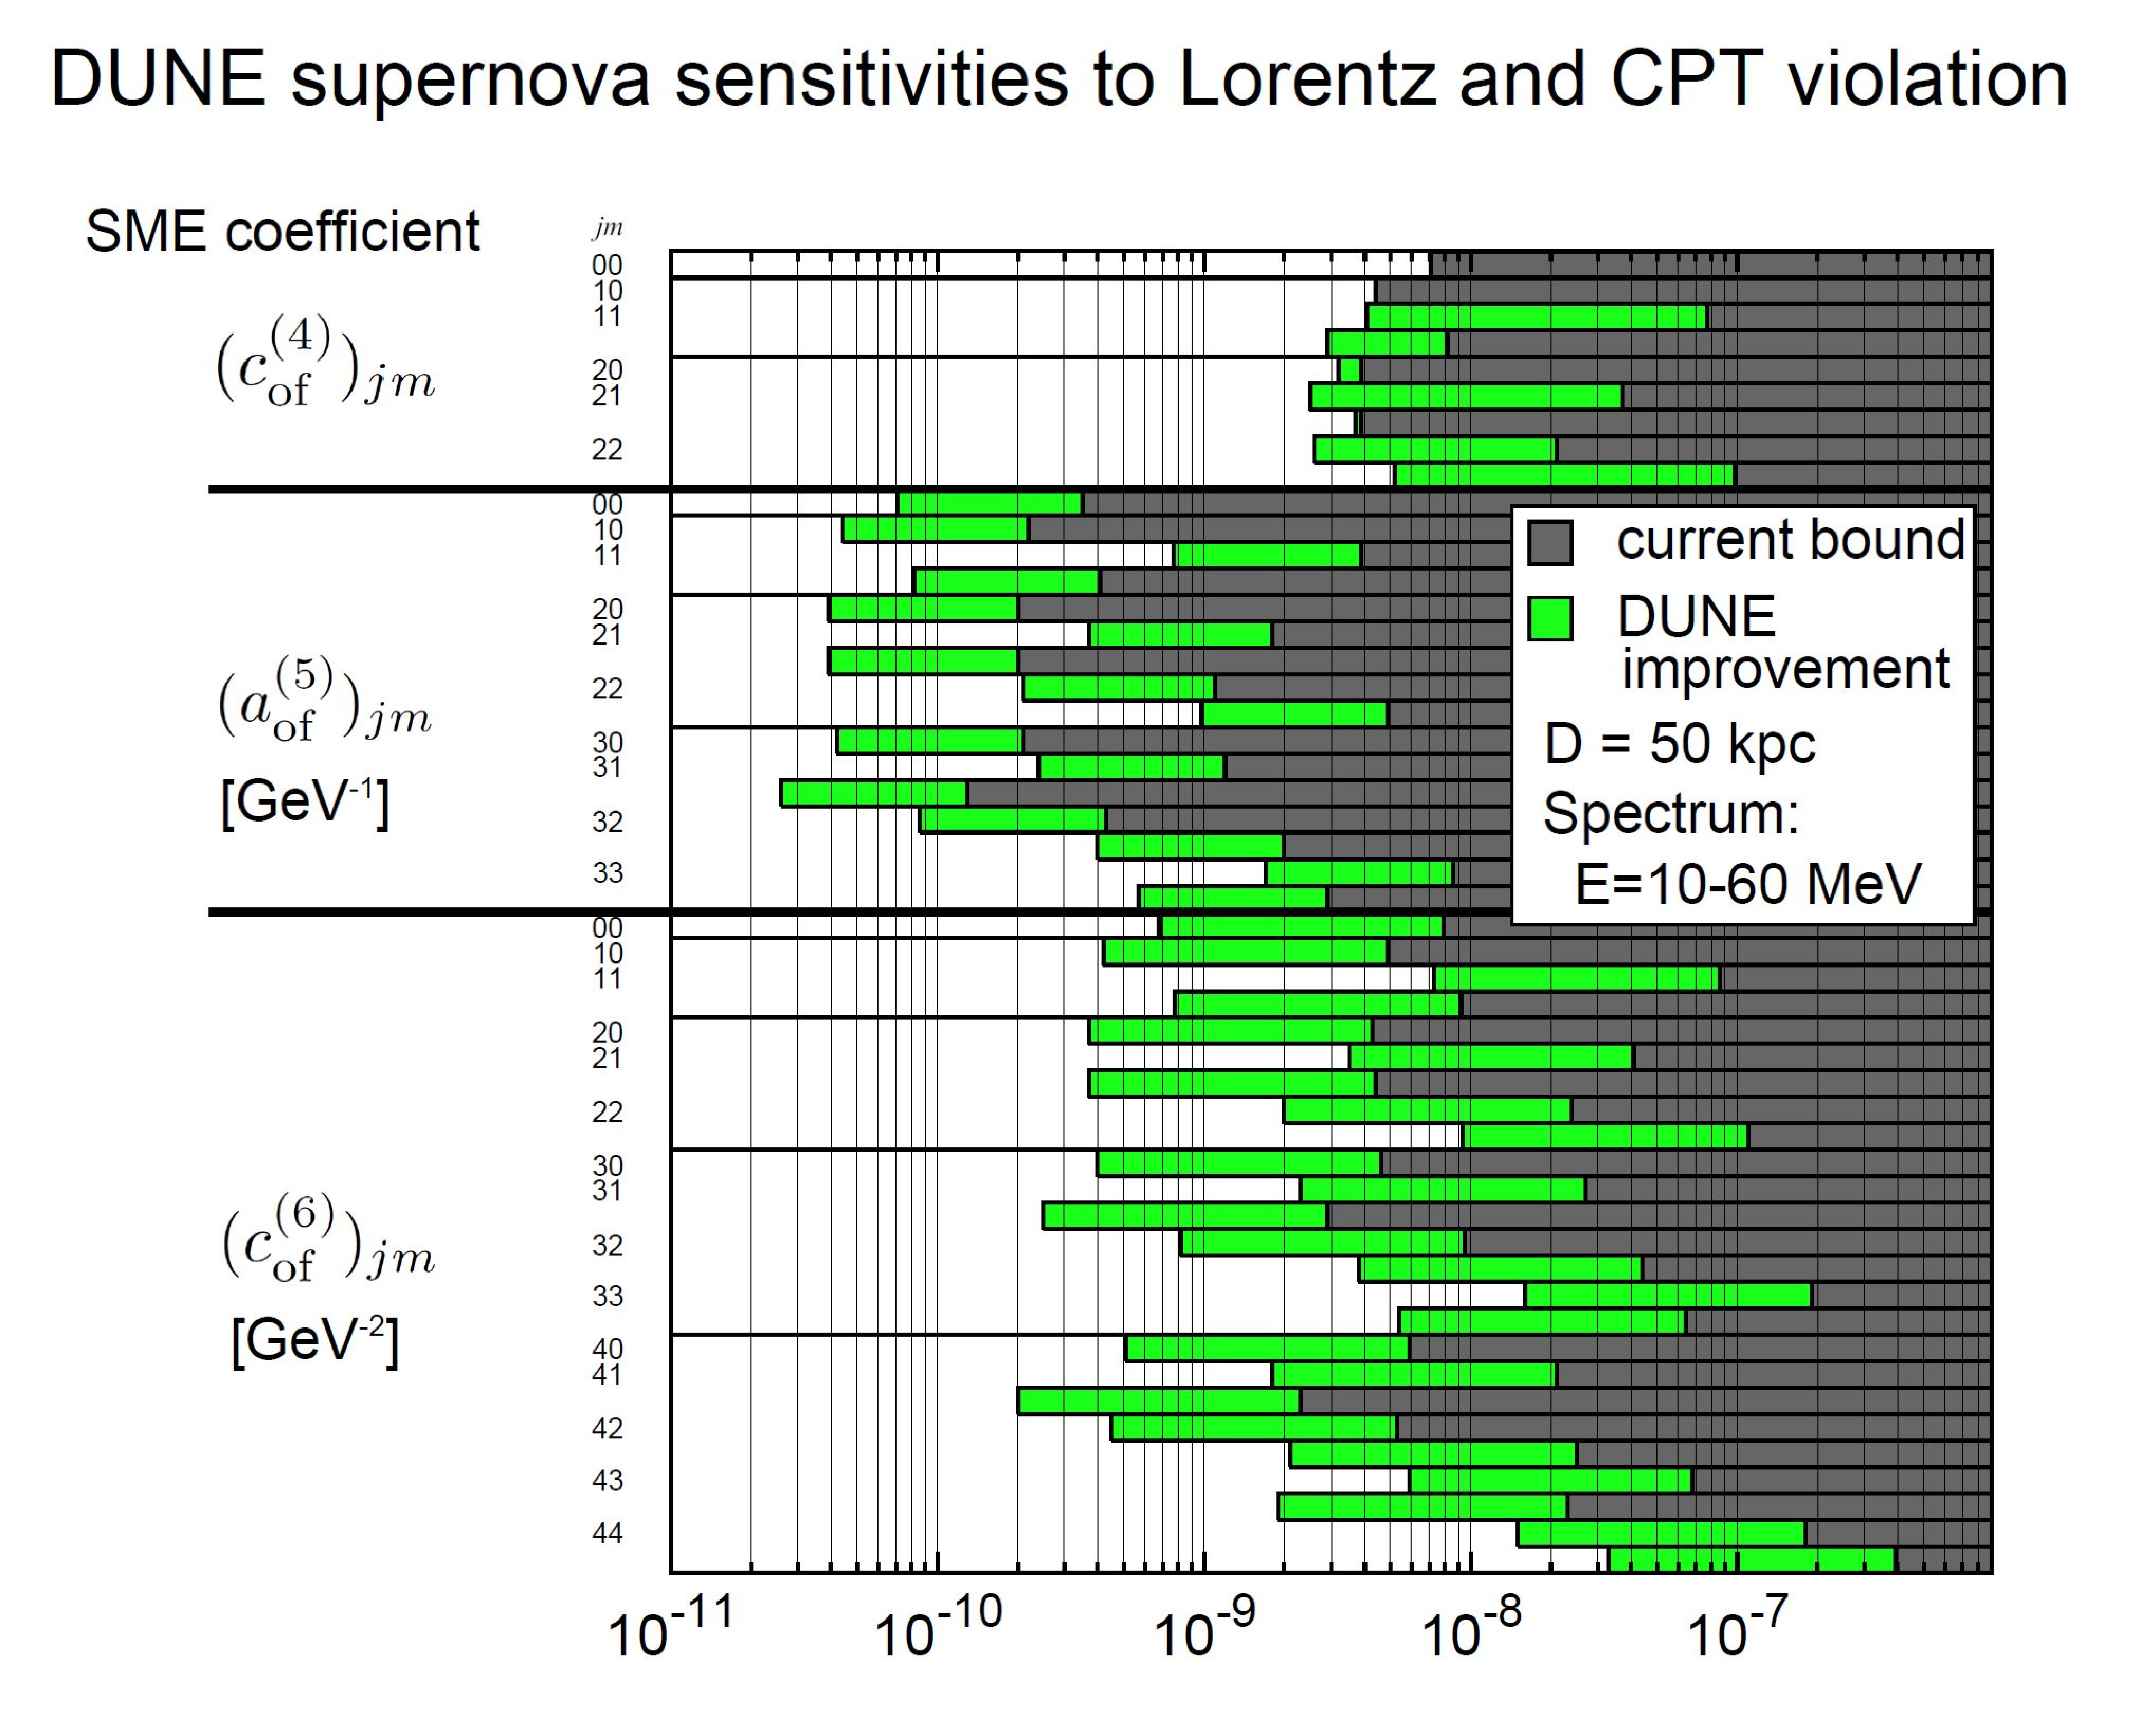
\includegraphics[width=0.9\textwidth]{DUNE-SME-SN.pdf}
\caption{DUNE supernova sensitivities to oscillation-free coefficients for Lorentz and CPT violation. Studies of DUNE supernova neutrinos can measure many coefficients (green) at levels improving over existing limits (grey). These Lorentz- and CPT- violating effects leave oscillations unchanged and so are unobservable in atmospheric or long-baseline measurements~\cite{alan}.}
\label{fig:snliv}
\end{figure}

% From Fernando Torres
Finally, via detection of time-of-flight delayed $\nu_e$ from the  neutronization burst,  DUNE will be able to probe neutrino mass bounds of $\mathcal{O}(1)$~eV for a 10-kpc supernova~\cite{Rossi-Torres:2015rla} (although likely not competitive near-future terrestrial kinematic limits).  If eV-scale sterile neutrinos exist, they will likely have an impact on astrophysical and oscillation aspects of the signal, as well as time-of-flight observables. \\


\section{Astrophysics}
\label{sec:physics-snblowe-astrophysics}


A number of astrophysical phenomena associated with supernovae are expected to be observable
in the supernova neutrino signal, providing a remarkable window into the event.  In particular, the supernova explosion mechanism, which in the current paradigm involves energy deposition via neutrinos, is still not well understood, and the neutrinos themselves will bring the insight needed to confirm or refute the paradigm.

There are many other examples of astrophysical observables.
\begin{itemize}
\item The initial burst, primarily composed of $\nu_e$ and called the
  ``neutronization'' or ``breakout''
  burst, %should be observable, although it
  represents only a small component of the total signal.  However,
  oscillation effects can manifest themselves in an observable manner
  in this burst, and flavor transformations can be modified by the
  ``halo'' of neutrinos generated in the supernova envelope by
  scattering~\cite{Cherry:2013mv}.
\item The formation of a black hole would cause a sharp signal cutoff
  (e.g.,~\cite{Beacom:2000qy,Fischer:2008rh}).
\item Shock wave effects (e.g.,~\cite{Schirato:2002tg}) would cause a
  time-dependent change in flavor and spectral composition as the
  shock wave propagates.
\item The standing accretion shock instability
  (SASI)~\cite{Hanke:2011jf,Hanke:2013ena}, a ``sloshing'' mode
  predicted by three-dimensional neutrino-hydrodynamics simulations of
  supernova cores, would give an oscillatory flavor-dependent
  modulation of the flux.
\item Turbulence effects~\cite{Friedland:2006ta,Lund:2013uta} would
  also cause flavor-dependent spectral modification as a function of
  time.
\end{itemize}

Observation of a supernova neutrino burst in coincidence with gravitational waves would be especially interesting~\cite{blah}.

The supernova neutrino burst is prompt with respect to the
electromagnetic signal and therefore can be exploited to provide an
early warning to astronomers~\cite{Antonioli:2004zb,Scholberg:2008fa}.  
Additionally, a liquid argon signal~\cite{Bueno:2003ei} is expected to
provide some pointing information, primarily from elastic scattering
on electrons.
We note that not every core collapse will produce an observable supernova, and observation of a neutrino burst in the absence of an electromagnetic event would be very interesting. 

Even non-observation of a burst, or non-observation of
a $\nu_e$ component of a burst in the presence of supernovae (or other
astrophysical events) observed in electromagnetic or gravitational
wave channels, would still provide valuable information about the
nature of the sources.  Further, a long-timescale, sensitive search
yielding no bursts will also provide limits on the rate of
core-collapse supernovae.


% r-process





\section{Additional Astrophysical Neutrinos}
\label{sec:physics-snblowe-other}

\subsection{Solar Neutrinos}

Intriguing questions in solar neutrino physics remain,
even after data
from the Super-K and SNO~\cite{Fukuda:2001nj,Ahmad:2001an}
experiments explained the long-standing mystery of missing solar
neutrinos~\cite{Cleveland:1998nv} as due to flavor
transformations. 
Some unknowns, such as the fraction of energy production via the CNO
cycle in the Sun, flux variation due to helio-seismological modes that
reach the solar core, or long-term stability of the solar core
temperature, are astrophysical in nature. Others directly impact
particle physics. Can the MSW model explain the amount of flavor
transformation as a function of energy, or are non-standard neutrino
interactions required?  Do solar neutrinos and reactor antineutrinos
oscillate with the same parameters? 
% Experimental data expected in the
%immediate future (e.g., further data from
%Borexino~\cite{Borexino7be:2011} and Super-K as well as 
%SNO+~\cite{Kraus:2006qp}) will address some questions, but the
%high-statistics measurements necessary to further constrain
%alternatives to the standard oscillation scenario may need to wait fo

Detection of solar and other low-energy neutrinos is challenging in
a LArTPC because of relatively high intrinsic detection energy thresholds for
the charged-current interaction on argon ($>$\SI{5}{\MeV}). 
%To be
%competitive, this physics requires either a very low visible energy
%threshold ($\sim$\SI{1}{\MeV}) or a very large mass (\SI{50}{\kt}).
Compared with other technologies, a LArTPC offers a large
cross section and unique potential signatures from de-excitation
photons. Aggressive R\&D efforts in low-energy triggering and
control of background from radioactive elements may make detection
of solar neutrinos in DUNE possible.
%, and a large detector mass would make the pursuit
%of these measurements worthwhile.

Signatures of solar neutrinos in DUNE
are elastic scattering on electrons as well as CC absorption of $\nu_e$ on $^{40}$Ar (equation~\ref{eq:nueabs}), which has a 4.5-MeV energy threshold.
In Table~\ref{tab:solarnu} the solar neutrino event rate in a
\ktadj{34} LArTPC is shown, assuming a \MeVadj{4.5} neutrino energy
threshold and 31\% $\nu_e$.
%
\begin{table}[!htb]
\caption[Solar neutrino rates in a LArTPC]{Solar neutrino event rates in a \ktadj{34} LArTPC assuming 
a \MeVadj{4.5} neutrino energy threshold and 31\% $\nu_e$ after oscillation.}
\label{tab:solarnu}
\begin{tabular}{$L^c}%$
\toprule
\rowtitlestyle
Transition & Rate (evts/day) \\ \toprowrule
Fermi  & 31 \\ \colhline
Gamow-Teller & 88 \\ \bottomrule
\end{tabular}
\end{table}


The solar neutrino physics potential of a large LArTPC depends
on the ability to pick up a low-energy electron, light collection of the photon-triggering system,
and, critically, on background suppression. 
Ihe decay of the naturally occurring $^{39}$Ar
produces $\beta$'s with a \keVadj{567} endpoint and an expected rate
of \SI{10}{\MHz} per \SI{10}{\kt} of liquid argon. This limits the
fundamental reach of DUNE to neutrino interactions with visible
energies above \SI{1}{\MeV}. 
Cosmic-muon and fast-neutrino  interactions with the $^{40}$Ar nucleus (which are rather complex
compared to interactions on $^{16}$O or $^{12}$C) are likely to generate many long-lived spallation products which could limit the
detection threshold for low-energy neutrinos.
% Studies of the spallation background in the DUNE LArTPC are
% underway. 
The production rate of $^{40}$Cl, a beta emitter with an
endpoint of \SI{7.48}{\MeV} that is a dominant source of background at
energies above \SI{5}{\MeV}, and is expected to be produced with a rate on the order of 10 per kton of LAr per day at 4850 ft.
% is shown in Figure~\ref{fig:cl40bkgd} as
% a function of depth.
% %
% \begin{figure}[!htb]
% \centering\includegraphics[width=0.7\textwidth]{figures/cosmicbkgd_40clrate.pdf}
% \caption[$^{40}$Cl production rates produced by (n,p) reaction per depth, \SI{10}{\kt}]{$^{40}$Cl production rates in a \ktadj{10} detector produced by (n,p) reaction as a function of depth.}
% \label{fig:cl40bkgd}
% \end{figure}
% %
% The cosmogenic background rates as a function of
% beta kinetic energy from several other beta emitters at the \SIadj{4850}{\ft} 
% level of Sanford Underground Research Facility are shown in Figure~\ref{fig:cosmicbkg}.
% %
% \begin{figure}[!htb]
% \centering
% \includegraphics[width=0.7\textwidth]{smyfig/solarmsw.pdf}
% \caption[Measurements of the solar MSW transition]{Measurements of the solar MSW transition. The red band combines
% SK and SNO $^8$B data~\cite{Aharmim:2011vm}, the green measurements
% of $^7$Be and pep are from Borexino~\cite{Borexino7be:2011,Borexinopep:2011} and the
% red error bar is Borexino's $^8$B measurement~\cite{Borexino8b:2008}. The 
% blue $pp$ point and the yellow error bar (CNO) combine all solar data. MSW resonance
% curves for three different parameters are overlaid.}
% \label{fig:solmsw}
% \end{figure}


The ICARUS collaboration has reported a \MeVadj{10}
threshold~\cite{Guglielmi:2012}. Assuming the %DUNE far 
detector itself
has low enough radioactivity levels, this threshold level would enable
a large enough detector to measure the electron flavor component of
the solar $^8$B neutrino flux with high statistical accuracy. It could % and
thereby further test the MSW flavor transformation curve with higher statistical precision and
potentially better energy resolution. 
In addition to these solar
matter effects, solar 
neutrinos also probe terrestrial matter effects
with the variation of the $\nu_e$ flavor observed with solar zenith
angle while the Sun is below the horizon --- the day/night effect (reported recently in ~\cite{Renshaw:2013dzu}). 
% A
% sizable effect is predicted only for the highest solar-neutrino
% energies, so while the comparatively high energy threshold is a
% handicap for testing the solar MSW resonance curve, it has a smaller
% impact on the high-statistics test of terrestrial matter
% effects. Recently, indication of the existence of the terrestrial
% matter effects were reported~\cite{Renshaw:2013}. Measurements of this
% effect currently give the best constraints on the solar mass ($\Delta
% m_{21}^2$) splitting 
% %(see Figure~\ref{fig:daynight}) 
% using neutrinos
% rather than antineutrinos~\cite{Gando:2013}.
%
% \begin{figure}[!htb]
% \centering\includegraphics[width=0.8\textwidth]{figures/sk_dn_vs_dm21.png}
% \caption[Solar neutrino day/night effect and dependence on $\Delta
% m^2_{21}$]{Dependence of the measured day/night asymmetry (fitted
%   day/night amplitude times the expected day/night asymmetry in red) on
%   $\Delta m^2_{21}$, for $\sin^2 \theta_{12}=0.314$ and $\sin^2
%   \theta_{13}=0.025$.  The 1$\sigma$ statistical uncertainties from
%   the recent measurements by \superk{} are given by the light
%   grey band. The additional dark grey width to the band shows the
%   inclusion of the systematic uncertainties. Overlaid are the 1$\sigma$ 
% allowed ranges from the solar global fit (solid green) and
%   the KamLAND experiment (dashed blue). Figure is courtesy of~\cite{Renshaw:2013}}
% \label{fig:daynight}
% \end{figure}
The comparison
of neutrino disappearance to antineutrino disappearance tests CPT
invariance. 
%For good sensitivity to either solar-neutrino measurement,
%a liquid argon far detector of at least \SI{34}{\kt} is required.


\subsection{Diffuse Supernova Background Neutrinos}

Galactic supernovae are relatively rare, occurring somewhere between
once and four times a century. In the Universe
at large, however, thousands of neutrino-producing explosions occur
every hour.  The resulting neutrinos --- in fact most of the neutrinos
%which have ever been 
emitted by all the supernovae since the onset of stellar formation ---
suffuse the Universe.  Know as the \emph{diffuse supernova neutrino background
  (DSNB)}, their energies are in the few-to-\MeVadj{30} range.  SRN
have not yet been observed, but an observation would greatly enhance
our understanding of supernova-neutrino emission and the overall
core-collapse rate.


A liquid argon detector such as DUNE's far detector is sensitive to
the $\nu_e$ component of the diffuse relic supernova neutrino flux,
whereas water Cherenkov and scintillator detectors are sensitive to
the antineutrino component.  However, backgrounds in liquid argon are as
yet unknown, and a huge exposure ($>$\SI{500}{\ktyr}s)
would likely be required for observation.  
%Given a detector of the
%scale required to achieve these exposures (\SIrange{50}{100}{\kt})
%together 
With tight control of
backgrounds, %with the appropriate technology,
DUNE --- in the long term --- could %eventually (Anne removed; redundant )
lay a unique and
 complementary role in the physics of relic neutrinos.

%
% In the current DUNE design, the irreducible background from solar
% neutrinos will limit the search for these relic neutrinos to an energy
% threshold greater than \SI{18}{MeV}.  Similarly, a search for relic
% antineutrinos is limited by the reactor antineutrino background to a
% threshold greater than $\sim$\SI{10}{MeV}. 
% The lower threshold and the
% smaller average $\nu_e$ energy relative to that for antineutrinos
% %\ (see
% %Figure~\ref{fig:pred_srnspec}) 
% leads to the need for a larger detector
% mass.

% A small but dedicated industry devotes itself to trying to predict the
% flux of these relic supernova neutrinos here on
% Earth~\cite{Totani:1995dw,Sato:1997sc,Hartmann:1997qe,Malaney:1996ar,Kaplinghat:1999xi,Ando:2005ka,Lunardini:2006pd,Fukugita:2002qw}. 
% Examples
% of two different predicted SRN spectra are shown in
% Figure~\ref{fig:pred_srnspec}, along with some of the key physics
% backgrounds from other neutrino sources.
% %
% \begin{figure}[!htb]
%      \centering\includegraphics[width=.8\textwidth]{smyfig/relicplot.pdf}
%      \caption[Relic supernova spectra and key neutrino
%      backgrounds]{Predicted relic supernova $\nu_e$ spectra from two
%        different models (red and blue) and some key neutrino
%        backgrounds: $^8$B solar $\nu_e$ (green), hep solar $\nu_e$
%        (cyan) and atmospheric $\nu_e$ (magenta).}
%      \label{fig:pred_srnspec}
% \end{figure}

% n the DUNE LArTPC, relic supernova electron neutrinos would be
% detected primarily via the charged current process as described by
% Equation~\ref{eqn:srninteract}. The electron track should be
% accompanied by evidence of ionization from the de-excitation of the
% potassium, e.g., shorter tracks sharing a common vertex; this is
% expected to help reduce backgrounds, but a detailed study has not yet
% been undertaken.  In water Cherenkov and scintillator detectors, it is
% the electron-antineutrino SRN flux that is detected through the
% process of inverse-beta decay.  Unlike inverse-beta decay, for which
% the cross section is known to the several-percent level in the energy
% range of interest~\cite{Vogel:1999zy,Strumia:2003zx}, the cross
% section for neutrino interactions on argon is uncertain at the 20\%
% level~\cite{Ormand:1994js,Kolbe:2003ys,SajjadAthar:2004yf}. Another
% limitation is that 
Background is a serious issue for DSNB detection.
The solar {\em hep} neutrinos, which have an                
endpoint at \SI{18.8}{\MeV}, will determine the lower bound of the DSNB
search window ($\sim$ \SI{16}{\MeV}).  The upper bound is determined
by the atmospheric ${\nu}_{e}$ flux and
%as shown in
%Figure~\ref{fig:pred_srnspec} and 
is around \SI{40}{MeV}.
%While the LArTPC provides a unique sensitivity
%to the electron-neutrino component of the SRN flux, early studies
%indicate that the lower bound on the neutrino energy imposed by solar
%neutrinos implies that a huge mass of LAr --- \SI{100}{\kt} --- is
%required to get more than 4$\sigma$ evidence for the diffuse supernova
%flux in five years~\cite{Cocco:2004ac}. 
Although the LArTPC provides a unique sensitivity to the
electron-neutrino component of the DSNB flux, early studies indicate
that due to this lower bound of $\sim$ \SI{16}{\MeV} DUNE would need a huge
mass of liquid argon --- of order \SI{100}{\kt} --- to get more than 4$\sigma$
evidence for the diffuse supernova flux in five
years~\cite{Cocco:2004ac}.
%
The expected number of relic
supernova neutrinos, $N_{\rm DSNB}$, that could be observed in a
\SIadj{40}{\kt} LArTPC detector in ten years~\cite{Cocco:2004ac}
assuming normal hierarchy is:
\begin{equation}
N_{\rm DSNB} = 46 \pm 10  \ \ \ 16 \, {\rm MeV} \leq E_e \leq 40 \, {\rm MeV}
\label{eqn:srnrate}
\end{equation}
where $E_e$ is the energy of the electron from the CC interaction as
shown in Equation~\ref{eq:nueabs}. 

% For 100 kt in 5 years was 57 \pm 12,  stat would be 7.5, so syst is 4.45/57 = 7.8%
% For 40 kt in 10 years, stat is 6.7, syst is 3.5568 so 46 \pm 10.

% The estimate of the SRN rate
% shown in Equation~\ref{eqn:srnrate} has a weak dependence on the value
% of $\sin ^2 \theta_{13}$. The above calculation is valid for values of
% $\sin ^2 \theta_{13} > 10^{-3}$. 
 The main challenge for detection of such
a low rate of relic neutrinos in a LArTPC is understanding how much of
the large spallation background from cosmic-ray interactions with the
heavy argon nucleus 
%(some of which are shown in Figure~\ref{fig:cosmicbkg}) 
leaks into the search window. 
%the rate is higher given that $\sin^2 \theta_{13}$ is an order of
%magnitude larger than originally estimated.

\subsection{Other Low-Energy Neutrino Sources}

We note some other potential sources of signals in the tens-of-MeV range which may be observable in DUNE.  These include neutrinos from accretion disks~\cite{Caballero:2011dw} and black-hole/neutron star mergers~\cite{Caballero:2009ww}.  These will create spectra not unlike those from core-collapse events, and with potentially large fluxes.  However they are expected to be considerably rarer than core-collapse supernovae within an observable distance range.
% \item ``Boosted'' dark matter?


\section{Detector Requirements and Capabilities for Low-Energy Events}
\label{sec:physics-snblowe-detector-requirements}

For supernova burst physics, the detector must be sensitive to energy depositions of at least 5 MeV.  It should also be capable of collecting information not only for a 10-kpc supernova, which would mean some thousands of events within 10 seconds, but also for a supernova at distances of less than 1 kpc, which would result in up to hundreds of thousands of events over 10 seconds, with a large fraction within the first second.    The detectors should be able to self-trigger on the burst, which may require sufficiently good photon detection, and provide prompt event information. 
The requirements for event reconstruction is that pointing back to the supernova should be limited primarily by event statistics rather than detector angular resolution.
Energy and event time resolution must be sufficient to resolve interesting physics features of the burst.  Preliminary studies suggest that resolution measured by Icarus for low-energy events~\cite{Amoruso:2003sw} should be adequate, and that approximately millisecond event time resolution should be sufficient to resolve features such as the neutronization burst and the preceding short notch due to neutrino trapping in the $\nu_e$ spectrum (see the luminosity curve of Fig.~\ref{fig:garching}), given adequate statistics.   Preliminary background studies (see Fig.~\ref{fig:vicbg}) show that cosmogenic and radioactive contaminants are likely to be subdominant for a Galactic burst; however backgrounds still need to be better understood for solar and DSNB signals.

\begin{figure}[htbp]
\begin{center}
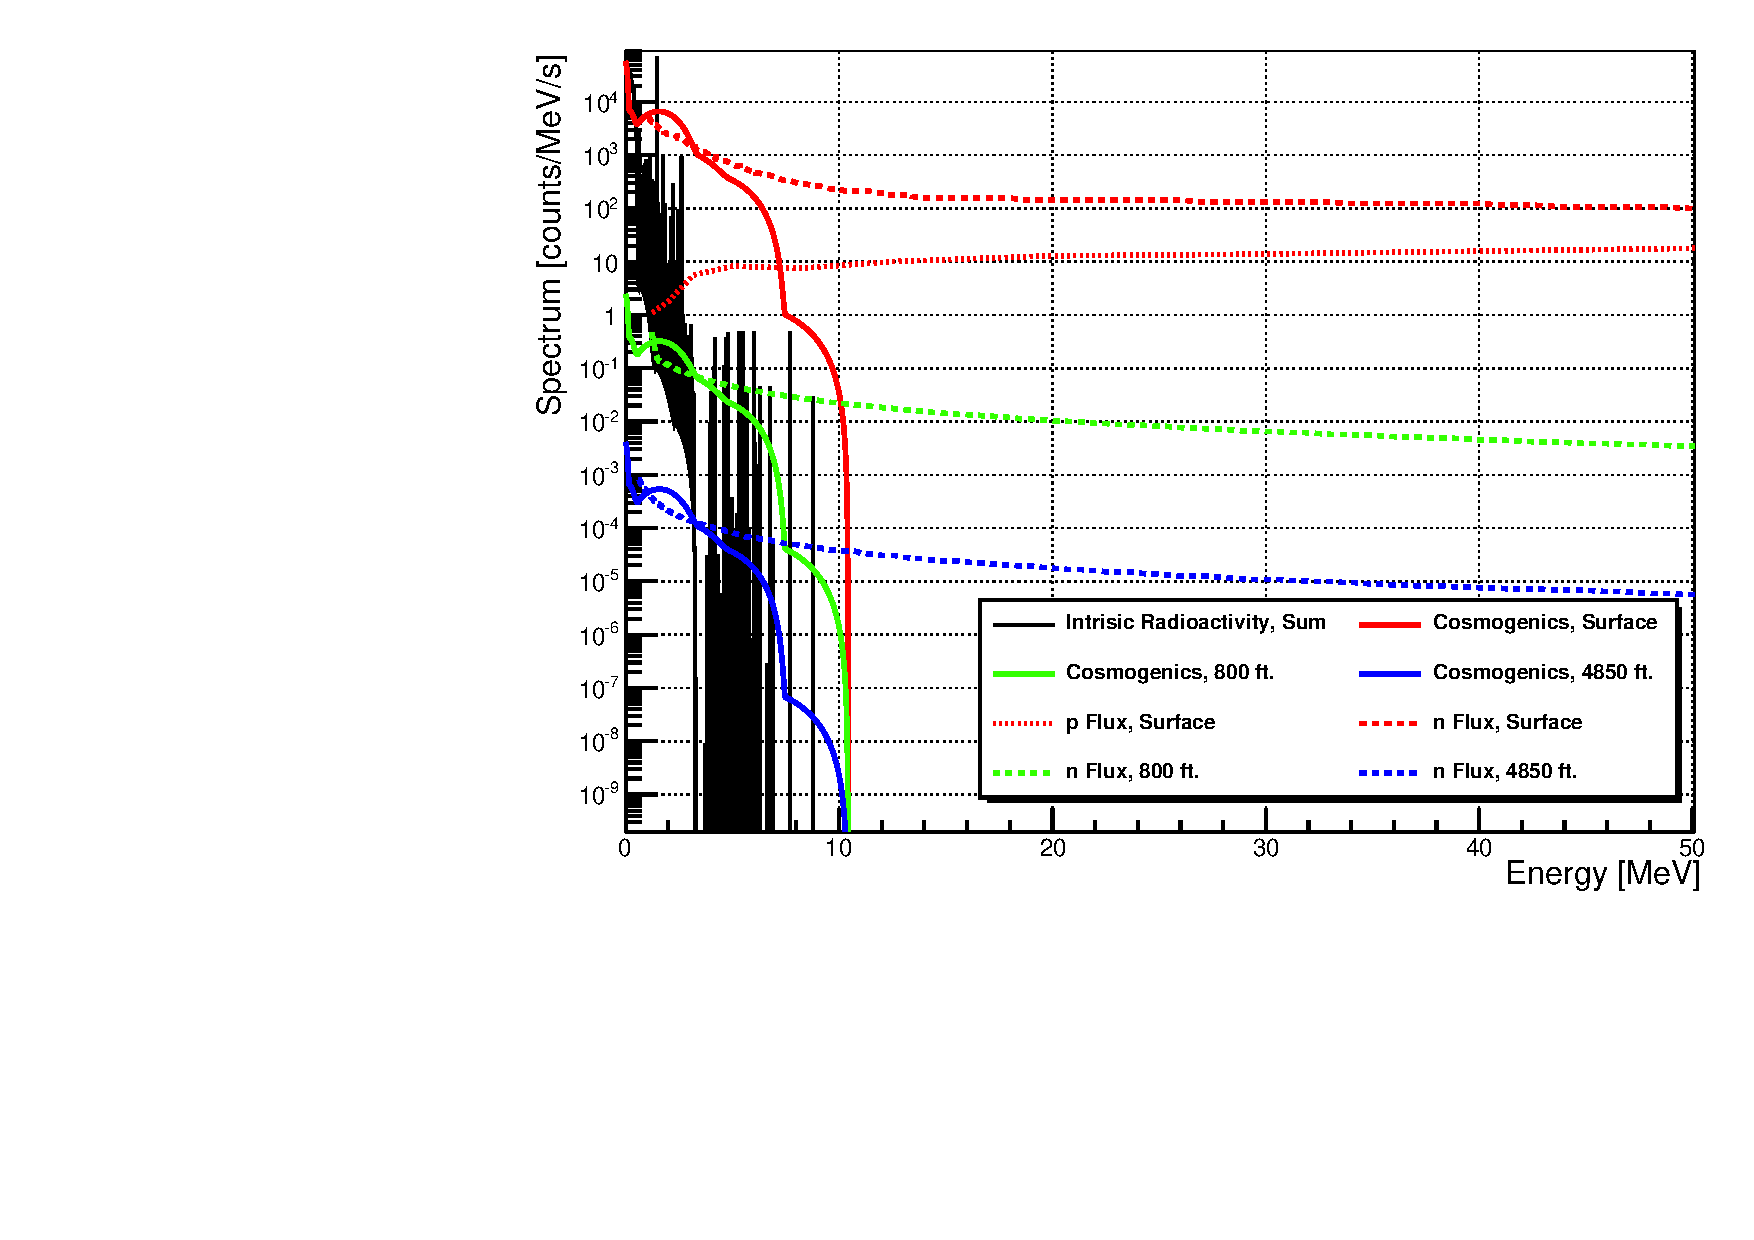
\includegraphics[width=12cm]{AllTheThings.pdf}
\caption{
All components of the background model used in a preliminary supernova background study, including radioactive decays (solid lines), cosmogenic neutron (dashed) and proton (dotted) fluxes.  The intrinsic background (independent of depth) is plotted in black.  Surface backgrounds are plotted in red, 800 feet of rock overburden in green, and 4850 feet in blue (color online). The rates are for 10 kton. } 
\label{fig:vicbg}
\end{center}
\end{figure}
\fixme{40 kt, typo in legend} 



Work is currently underway using the LArSoft simulation package
to characterize low-energy
response for realistic DUNE detector configurations.
%Figure~\ref{fig:evdisplays} shows a sample \MeVadj{20} event in the DUNE
%\SIadj{35}{t} prototype
%\ktadj{10} 
%geometry simulated with LArSoft. 
So far,
most studies have been done with the MicroBooNE geometry, with the
results expected to be %largely
generally applicable to the larger DUNE detectors.  For a preliminary
understanding of achievable energy resolution, isotropic and uniform
monoenergetic electrons with energies of 5-50~MeV (which should
approximate the $\nu_e$-CC electron products) were simulated and
reconstructed with the LArSoft
package. 
The charge of reconstructed hits on the collection plane was used to
reconstruct the energy of the primary electrons. (Induction-plane charge
as well as track-length-based reconstruction were also considered, but
with inferior results). Figure~\ref{fig:lowe_res} shows the results of a resolution study (see caption).
A correction to compensate for loss of electrons during drift,
$Q_{collection}=Q_{production}\times e^{-T_{\rm drift} / T_{\rm
    electron}}$ (where $T_{drift}$ is the drift time of the ionization
electrons, and $T_{electron}$ is the electron lifetime), using Monte
Carlo truth to evaluate $T_{\rm drift}$, improved resolution
significantly.  This study indicated that photon time information will
be valuable for low-energy event reconstruction.  Some of the
resolution was determined to be due to imperfect hit-finding by the
nominal reconstruction software.  A tuned hit-finding algorithm did
somewhat better (Figure~\ref{fig:lowe_res}), and further
improvements for reconstruction algorithms optimized for low-energy
events are expected.
%
% \begin{figure}[!htb]
% \begin{centering}
%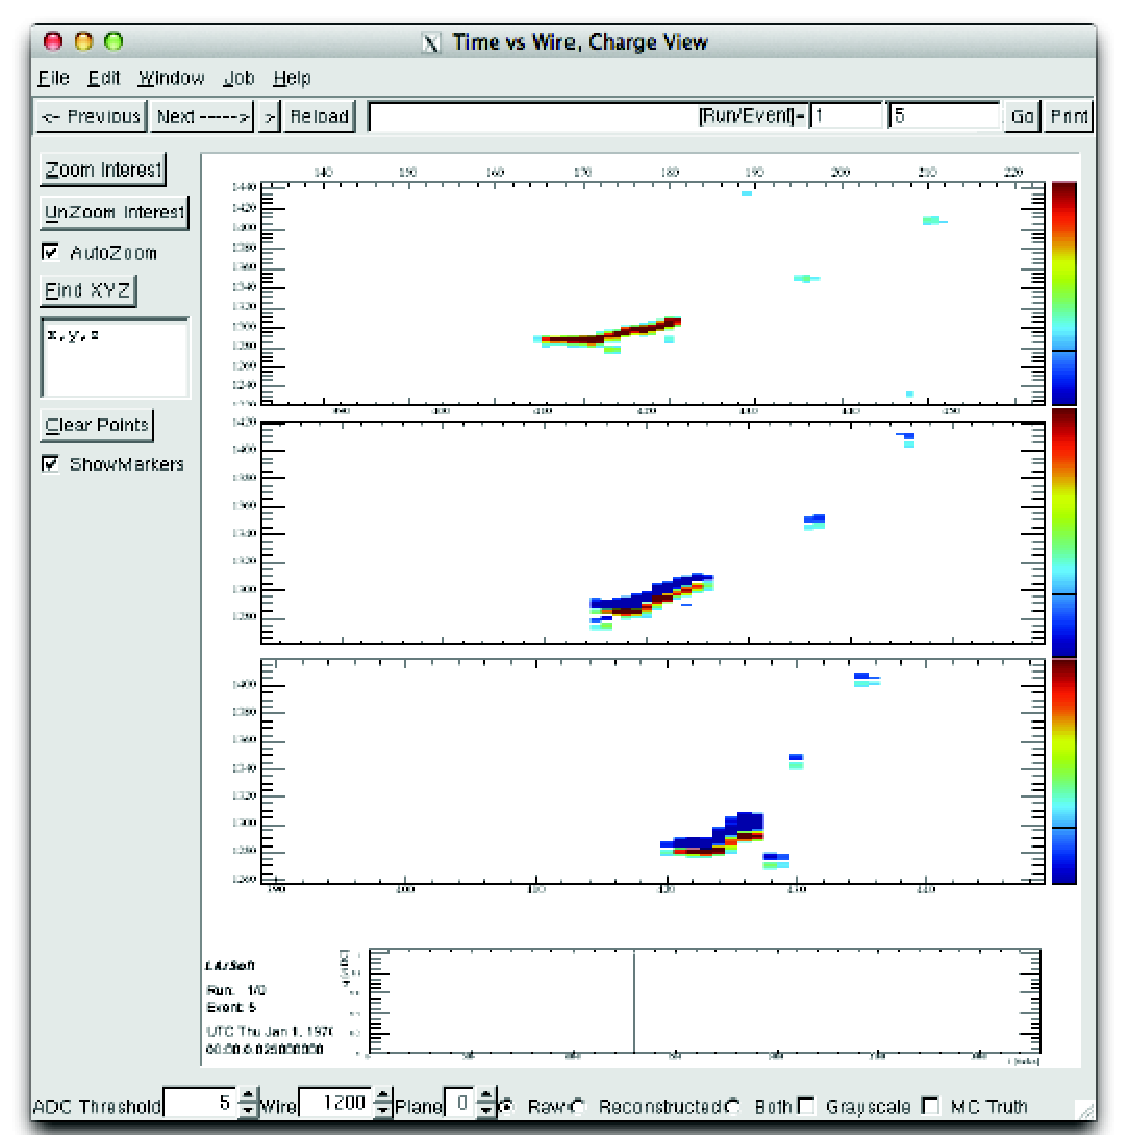
\includegraphics[height=2.5in]{snfig/15MeV_fixedvertexdir.pdf}
% 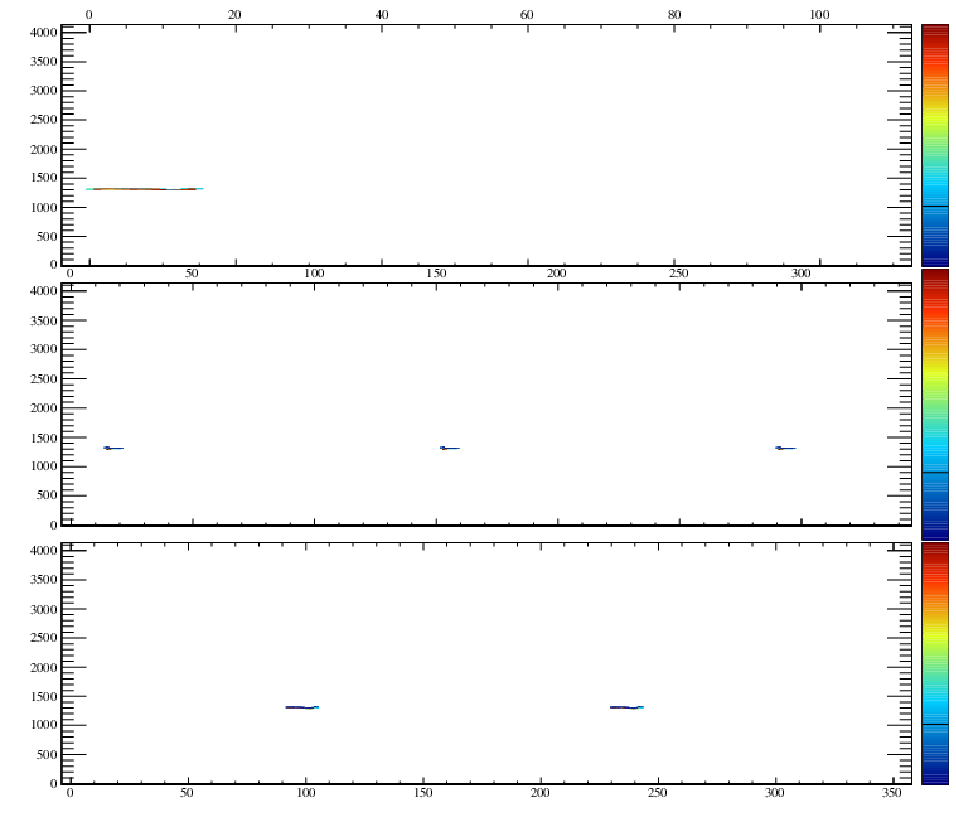
\includegraphics[width=0.9\textwidth]{snfig/elect20mev35tunzoom_mod.pdf}
% %\includegraphics[width=0.4\textwidth,bb=0 -200 600 1000]{snfig/lbne_zoom.pdf}
% %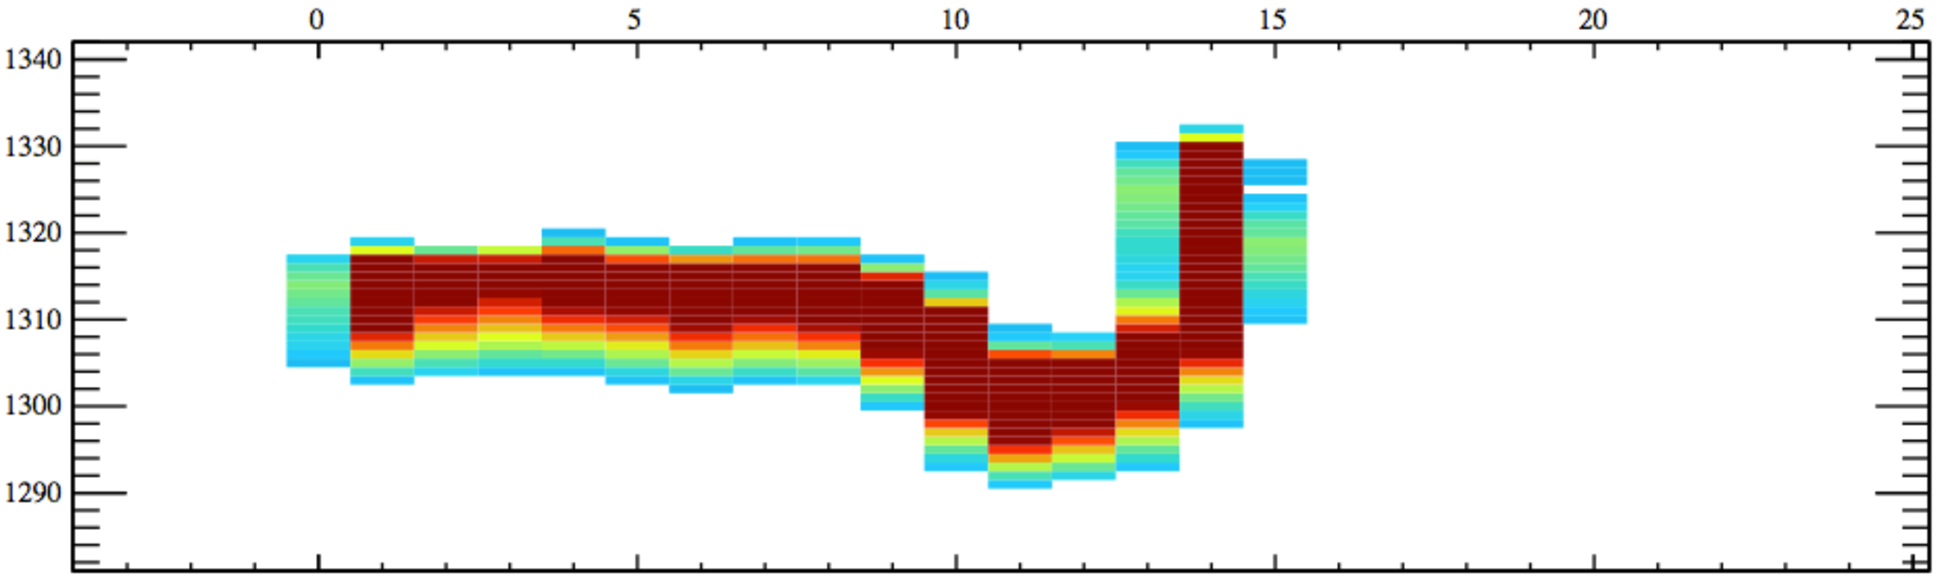
\includegraphics[width=0.84\textwidth]{snfig/elect20mev35tzoomcropped.pdf}
% \caption[Typical \MeVadj{20} event in the DUNE
%   \SIadj{35}{t} prototype geometry]{Raw event display of a simulated \MeVadj{20} event in the DUNE
%   \SIadj{35}{t} prototype; the top panel shows the collection plane, and the
%   lower two panels show the induction planes (with multiple images due
%   to wire wrapping). The bottom panel shows a zoom of the collection plane image.
%  }
% \label{fig:evdisplays}
% \end{centering}
% \end{figure}
%
\begin{figure}[!htb] %  figure placement: here, top, bottom, or page
 \centering
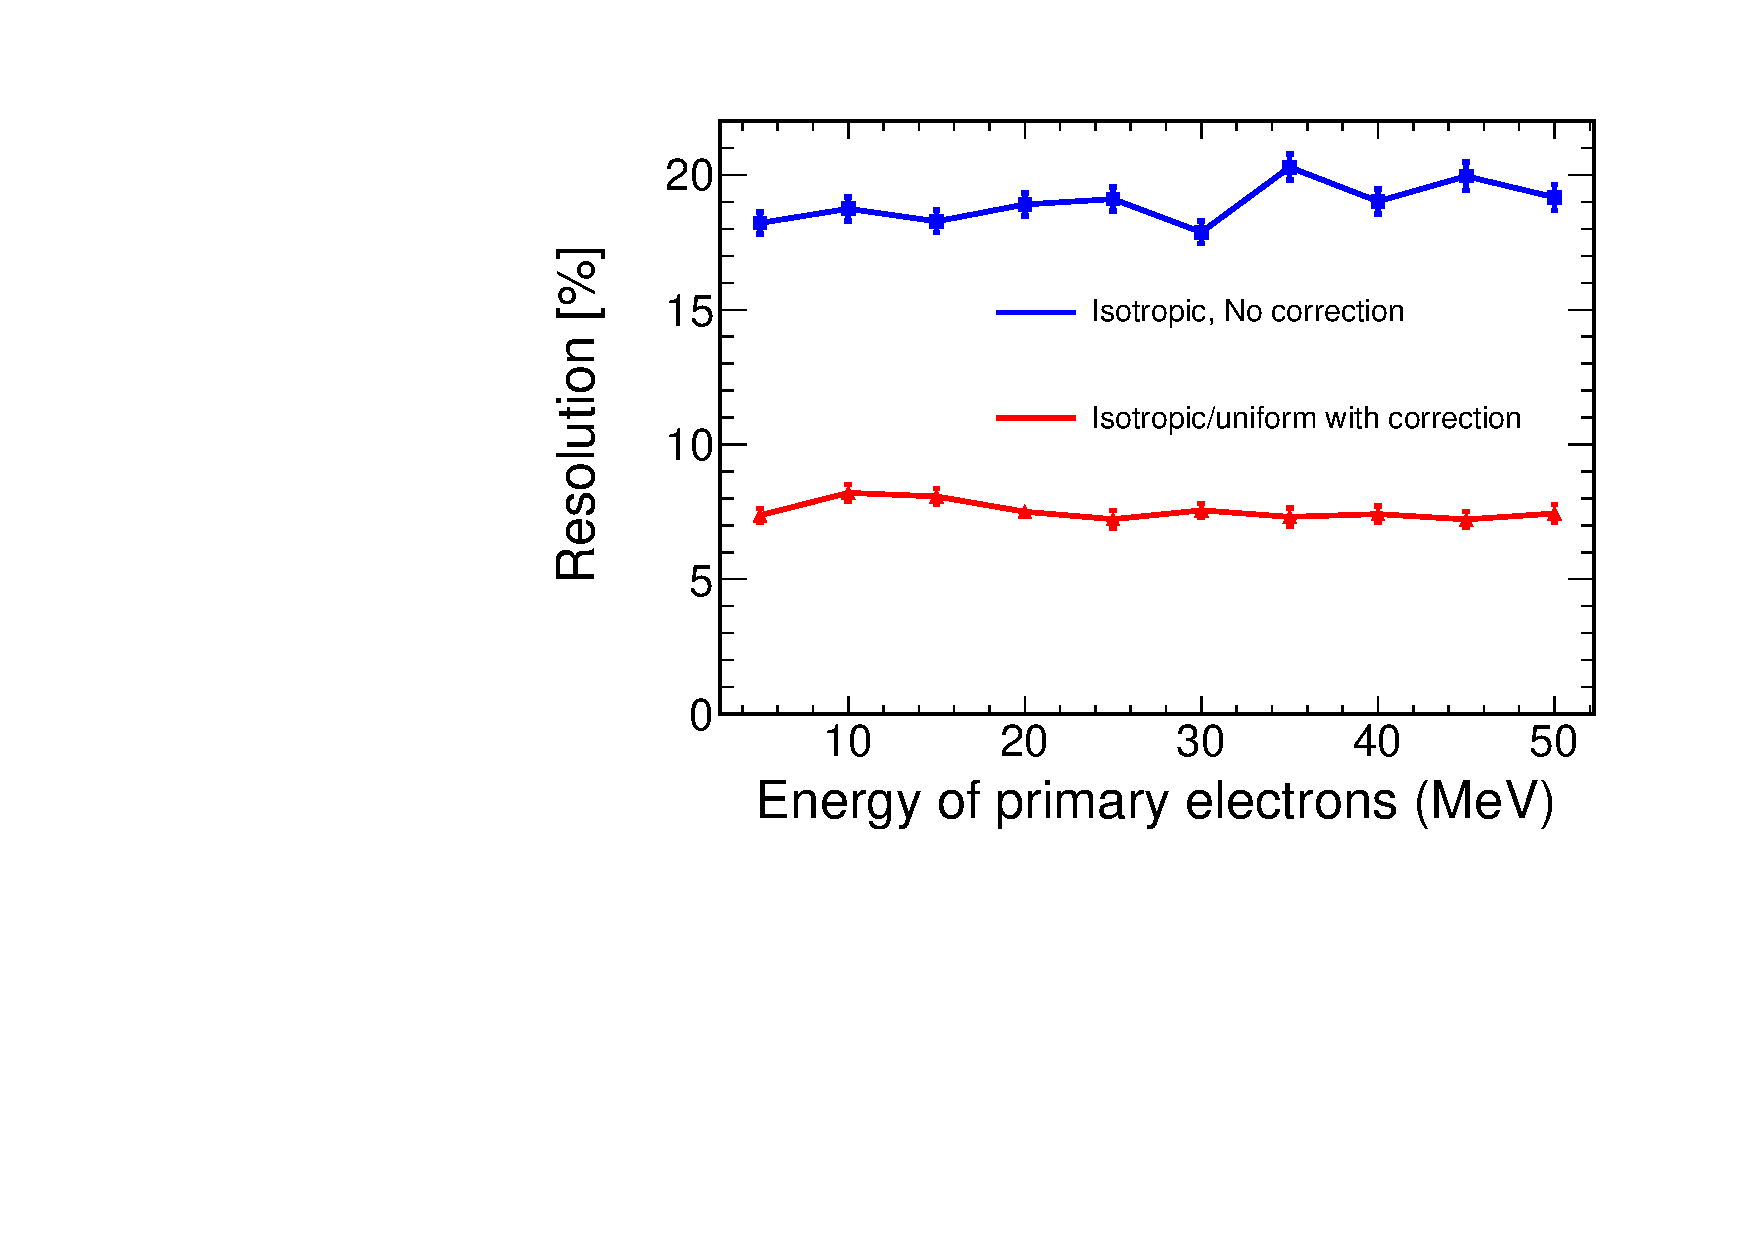
\includegraphics[width=0.45\textwidth]{correction.pdf} 
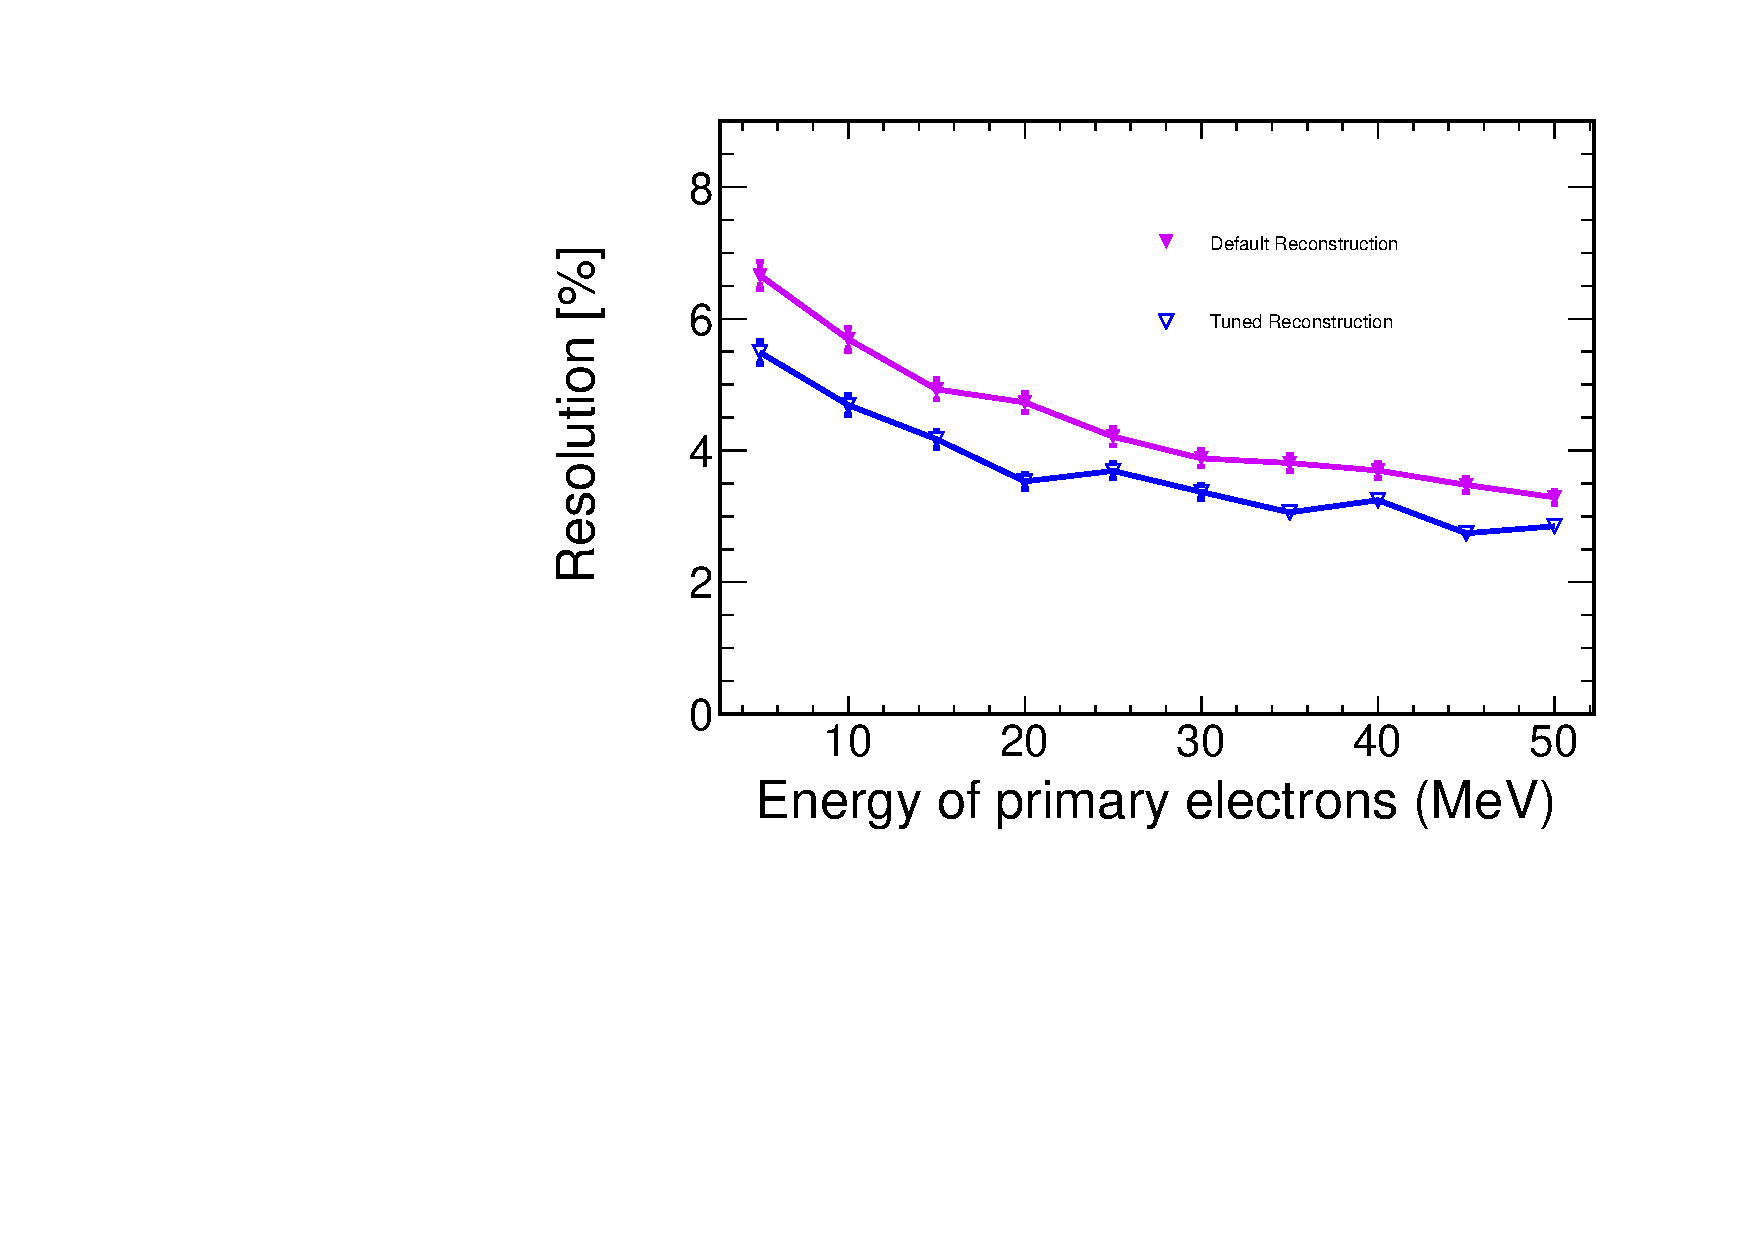
\includegraphics[width=0.45\textwidth]{hitfinder.pdf} 

 \caption[Comparisons of energy resolution]{Left: Comparison of energy
   resolution (defined as $\sigma/E$, where $\sigma$ is the spread of
   the collection-plane-charge-based event energy $E$ for a
   monoenergetic electron), with and without electron-lifetime
   correction, as a function of electron energy. The blue curve is the
   energy resolution of isotropic and uniform electrons without
   electron-lifetime correction. The red curve is the energy
   resolution with electron-lifetime correction based on MC truth.
   Right: Comparison of energy resolution before and after tuning the
   reconstruction algorithm (for fixed position/direction electron
   events).}\label{fig:lowe_res}
\end{figure}


%Preliminary
%results show that energy resolutions 
%for baseline detector parameters
%will not differ too significantly from those in~\cite{Amoruso:2003sw}.
Also under study is the potential for tagging $\nu_e$-CC absorption
events ($\nu_e +{}^{40}{\rm Ar} \rightarrow e^- +{}^{40}{\rm
  K^*}$) using the cascade of de-excitation $\gamma$ rays (which Compton-scatter in the detector), which should
serve the dual purposes of rejecting background and isolating the CC
component of the signal.  Reconstructing these gammas also improves the neutrino energy measurement. 


